% oil_geilo_2014.tex

%Presentation at IFN, November 2013

\documentclass{beamer}

\usepackage{amsmath}
\usepackage{esdiff} %for writing partial derivatives
\usetheme{default}

\title[OIL]{The Decline of Norwegian Oil}
\subtitle[Errors]{The Effect of Price on Production in a Mature Petroleum Region}
\author[J. Mauritzen]{Johannes Mauritzen}
\institute[NHH]{
 % Department of Business and Management Science\\
 % NHH Norwegian School of Economics\\[1ex]
  \texttt{johannes.mauritzen@nhh.edu}
}
\date[Feb 2014]{February 2014}

\begin{document}

%--- the titlepage frame -------------------------%
\begin{frame}[plain]
  \titlepage
\end{frame}


%--- the presentation begins here ----------------%

%--- Intro 						  ----------------%
%--- the presentation begins here ----------------%

\begin{frame}[plain]
	\begin{itemize}

	\item Effect of Price on Drilling / Reserve Replacement
	\begin{itemize} \item Mohn and Osmundsen (2008), Mohn (2008), Ringlund (2008) \end{itemize}
	 \item Production (Aggregate)

		\begin{itemize}
		\item Curve-fitting/Simulation (geo-engineering)
		\item Econometric
			\begin{itemize}
			\item Kaufman (1990), Kaufman and Cleveland (2001)
			\item Ramcharran (2002):  Negative Price Elasticity (???)
	 		\end{itemize}
	 	\end{itemize}
	\end{itemize}
\end{frame}

\begin{frame}[plain]
Generalized Additive Models
\begin{itemize}
\item  Hastie and Tibshirani (1990) 
\item  Wood (2006)
\end {itemize}

\end{frame}

\begin{frame}[plain]
Main Results
\begin{itemize}
\item  No significant contemporary effect of oil price on field production (within 3 years)
\item Slight lagged effect found after 4-8 years, magnitude of around 2\%
\item Most of this effect seems to come in the Planning stage of an oil field
\item Little to no effect - contemporary or lagged - in depleting fields
\end {itemize}

\end{frame}

\begin{frame}[plain]
	\begin{figure}
	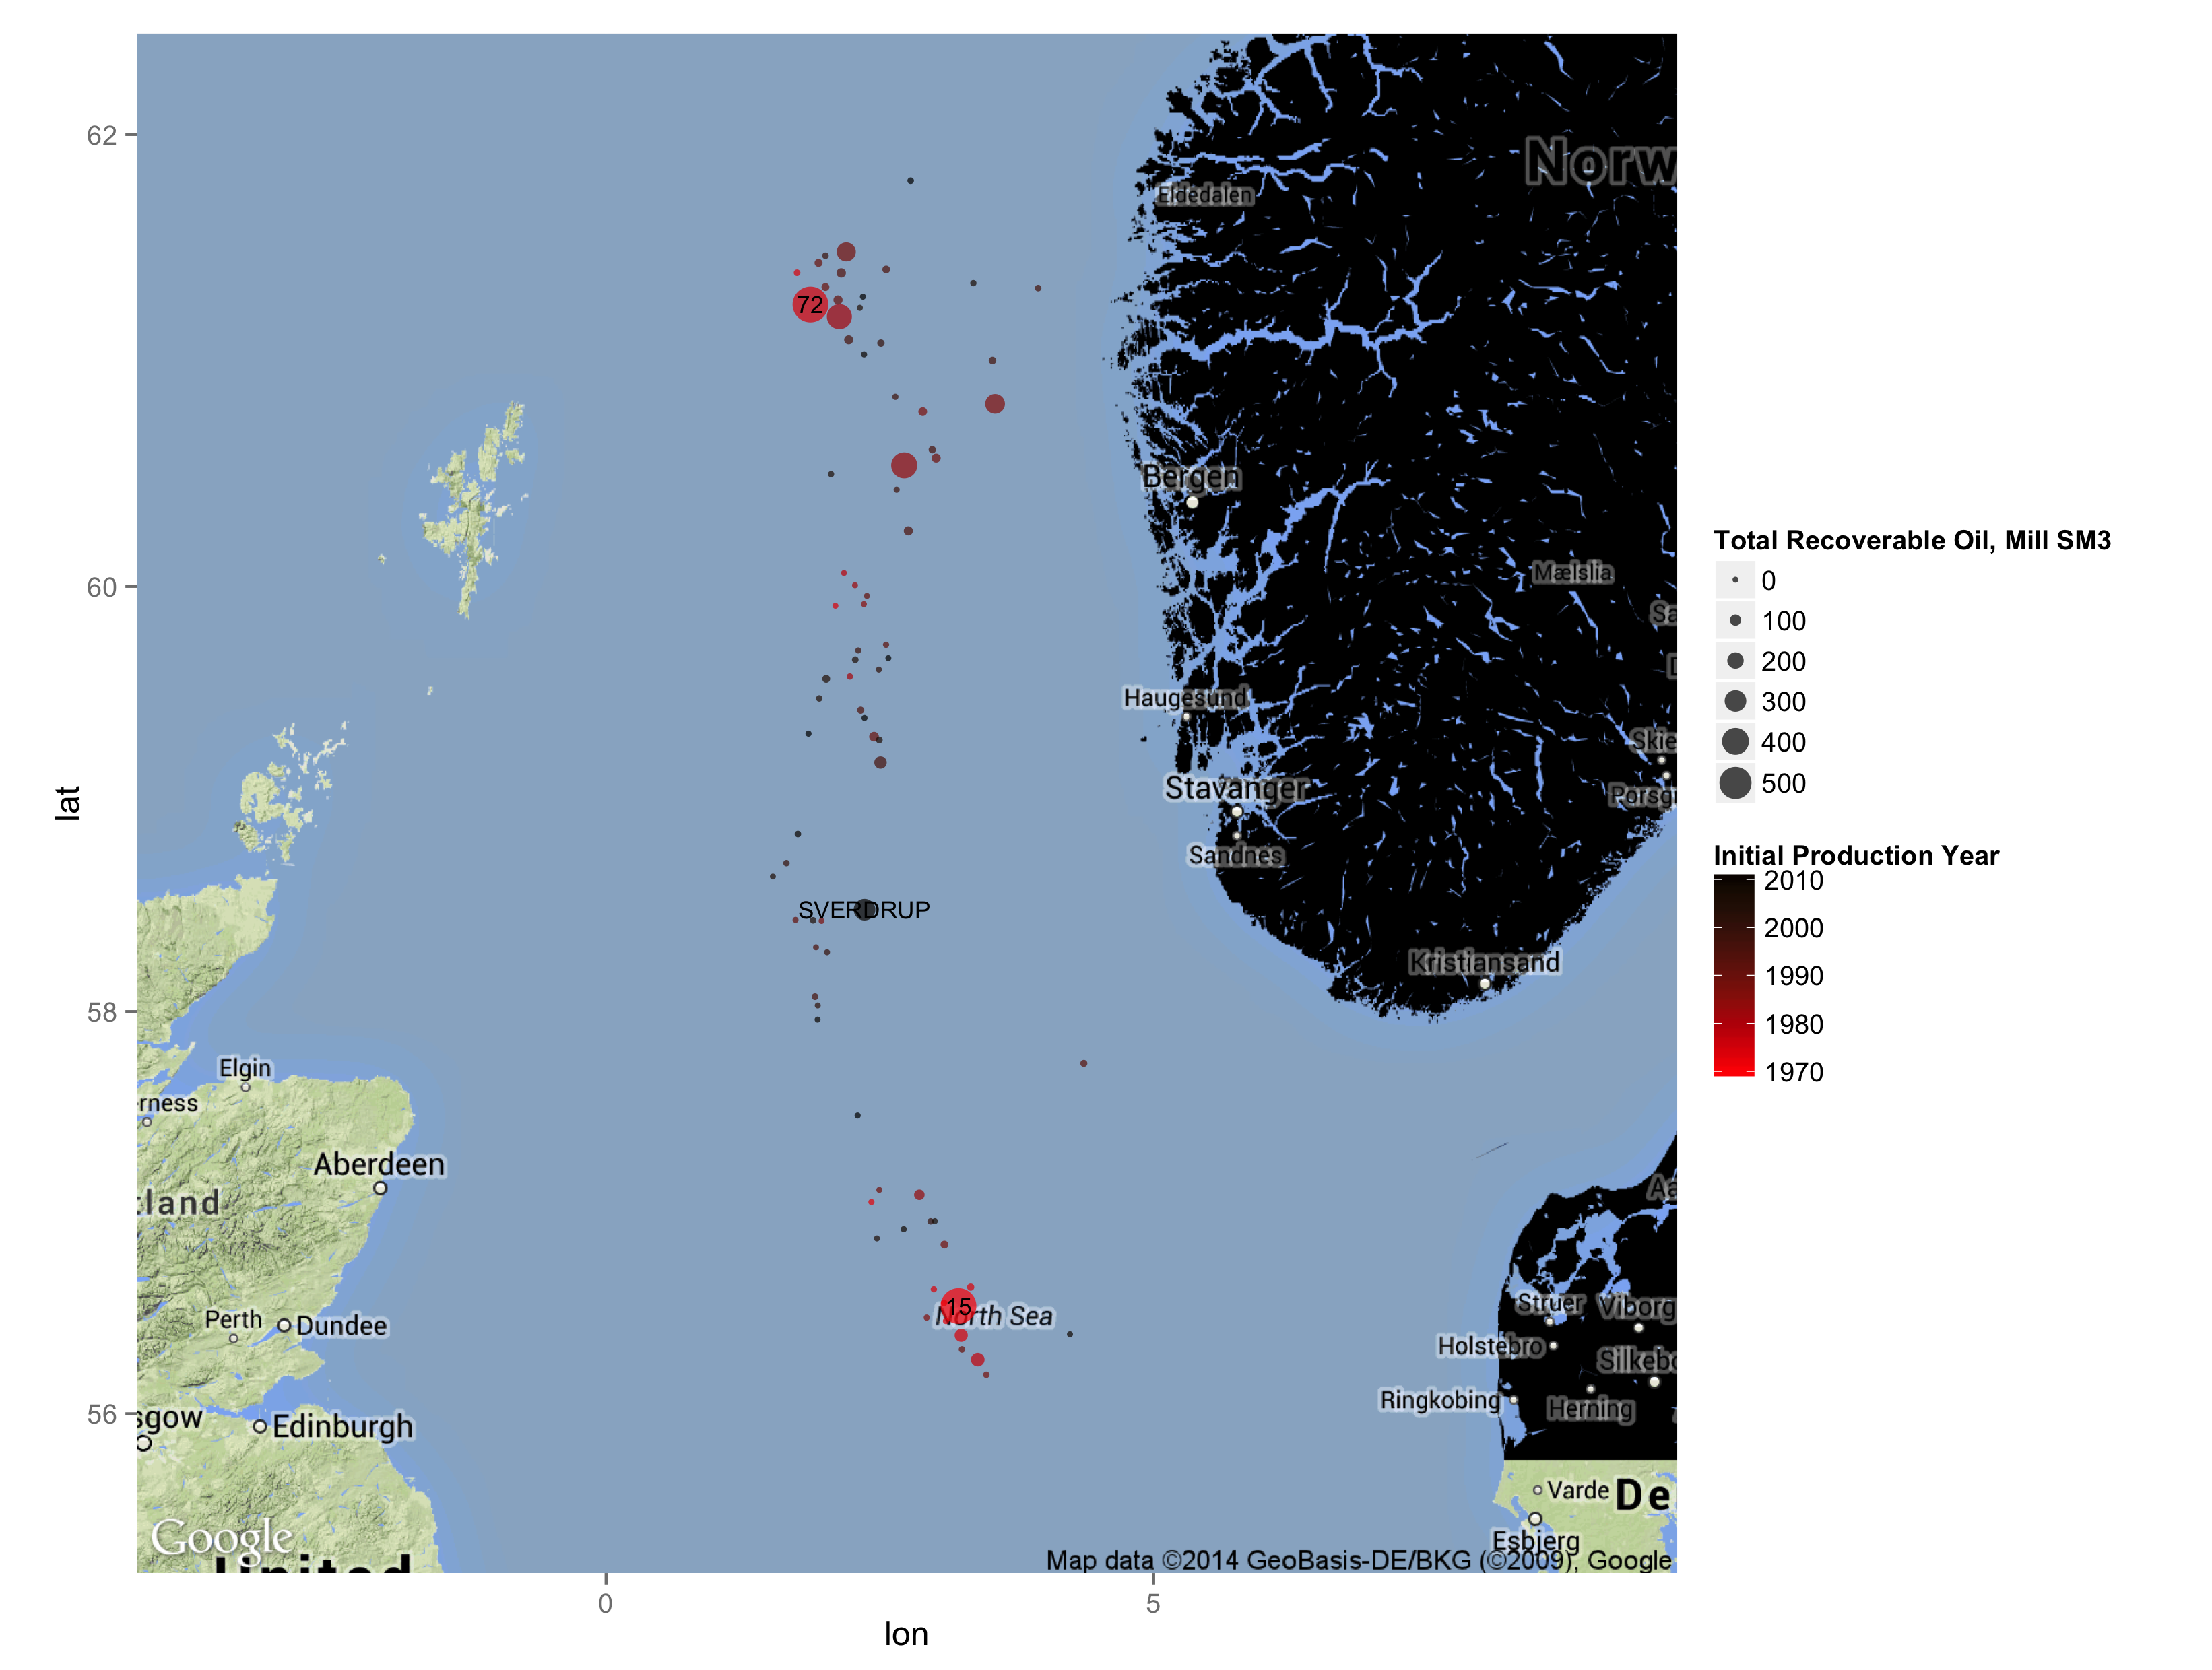
\includegraphics[width=.8\textwidth]{figures/north_sea_reserves.png}
	\caption*{}
	\label{north_sea_reserves}
	\end{figure}
\end{frame}


\begin{frame}[plain]
	\begin{figure}
	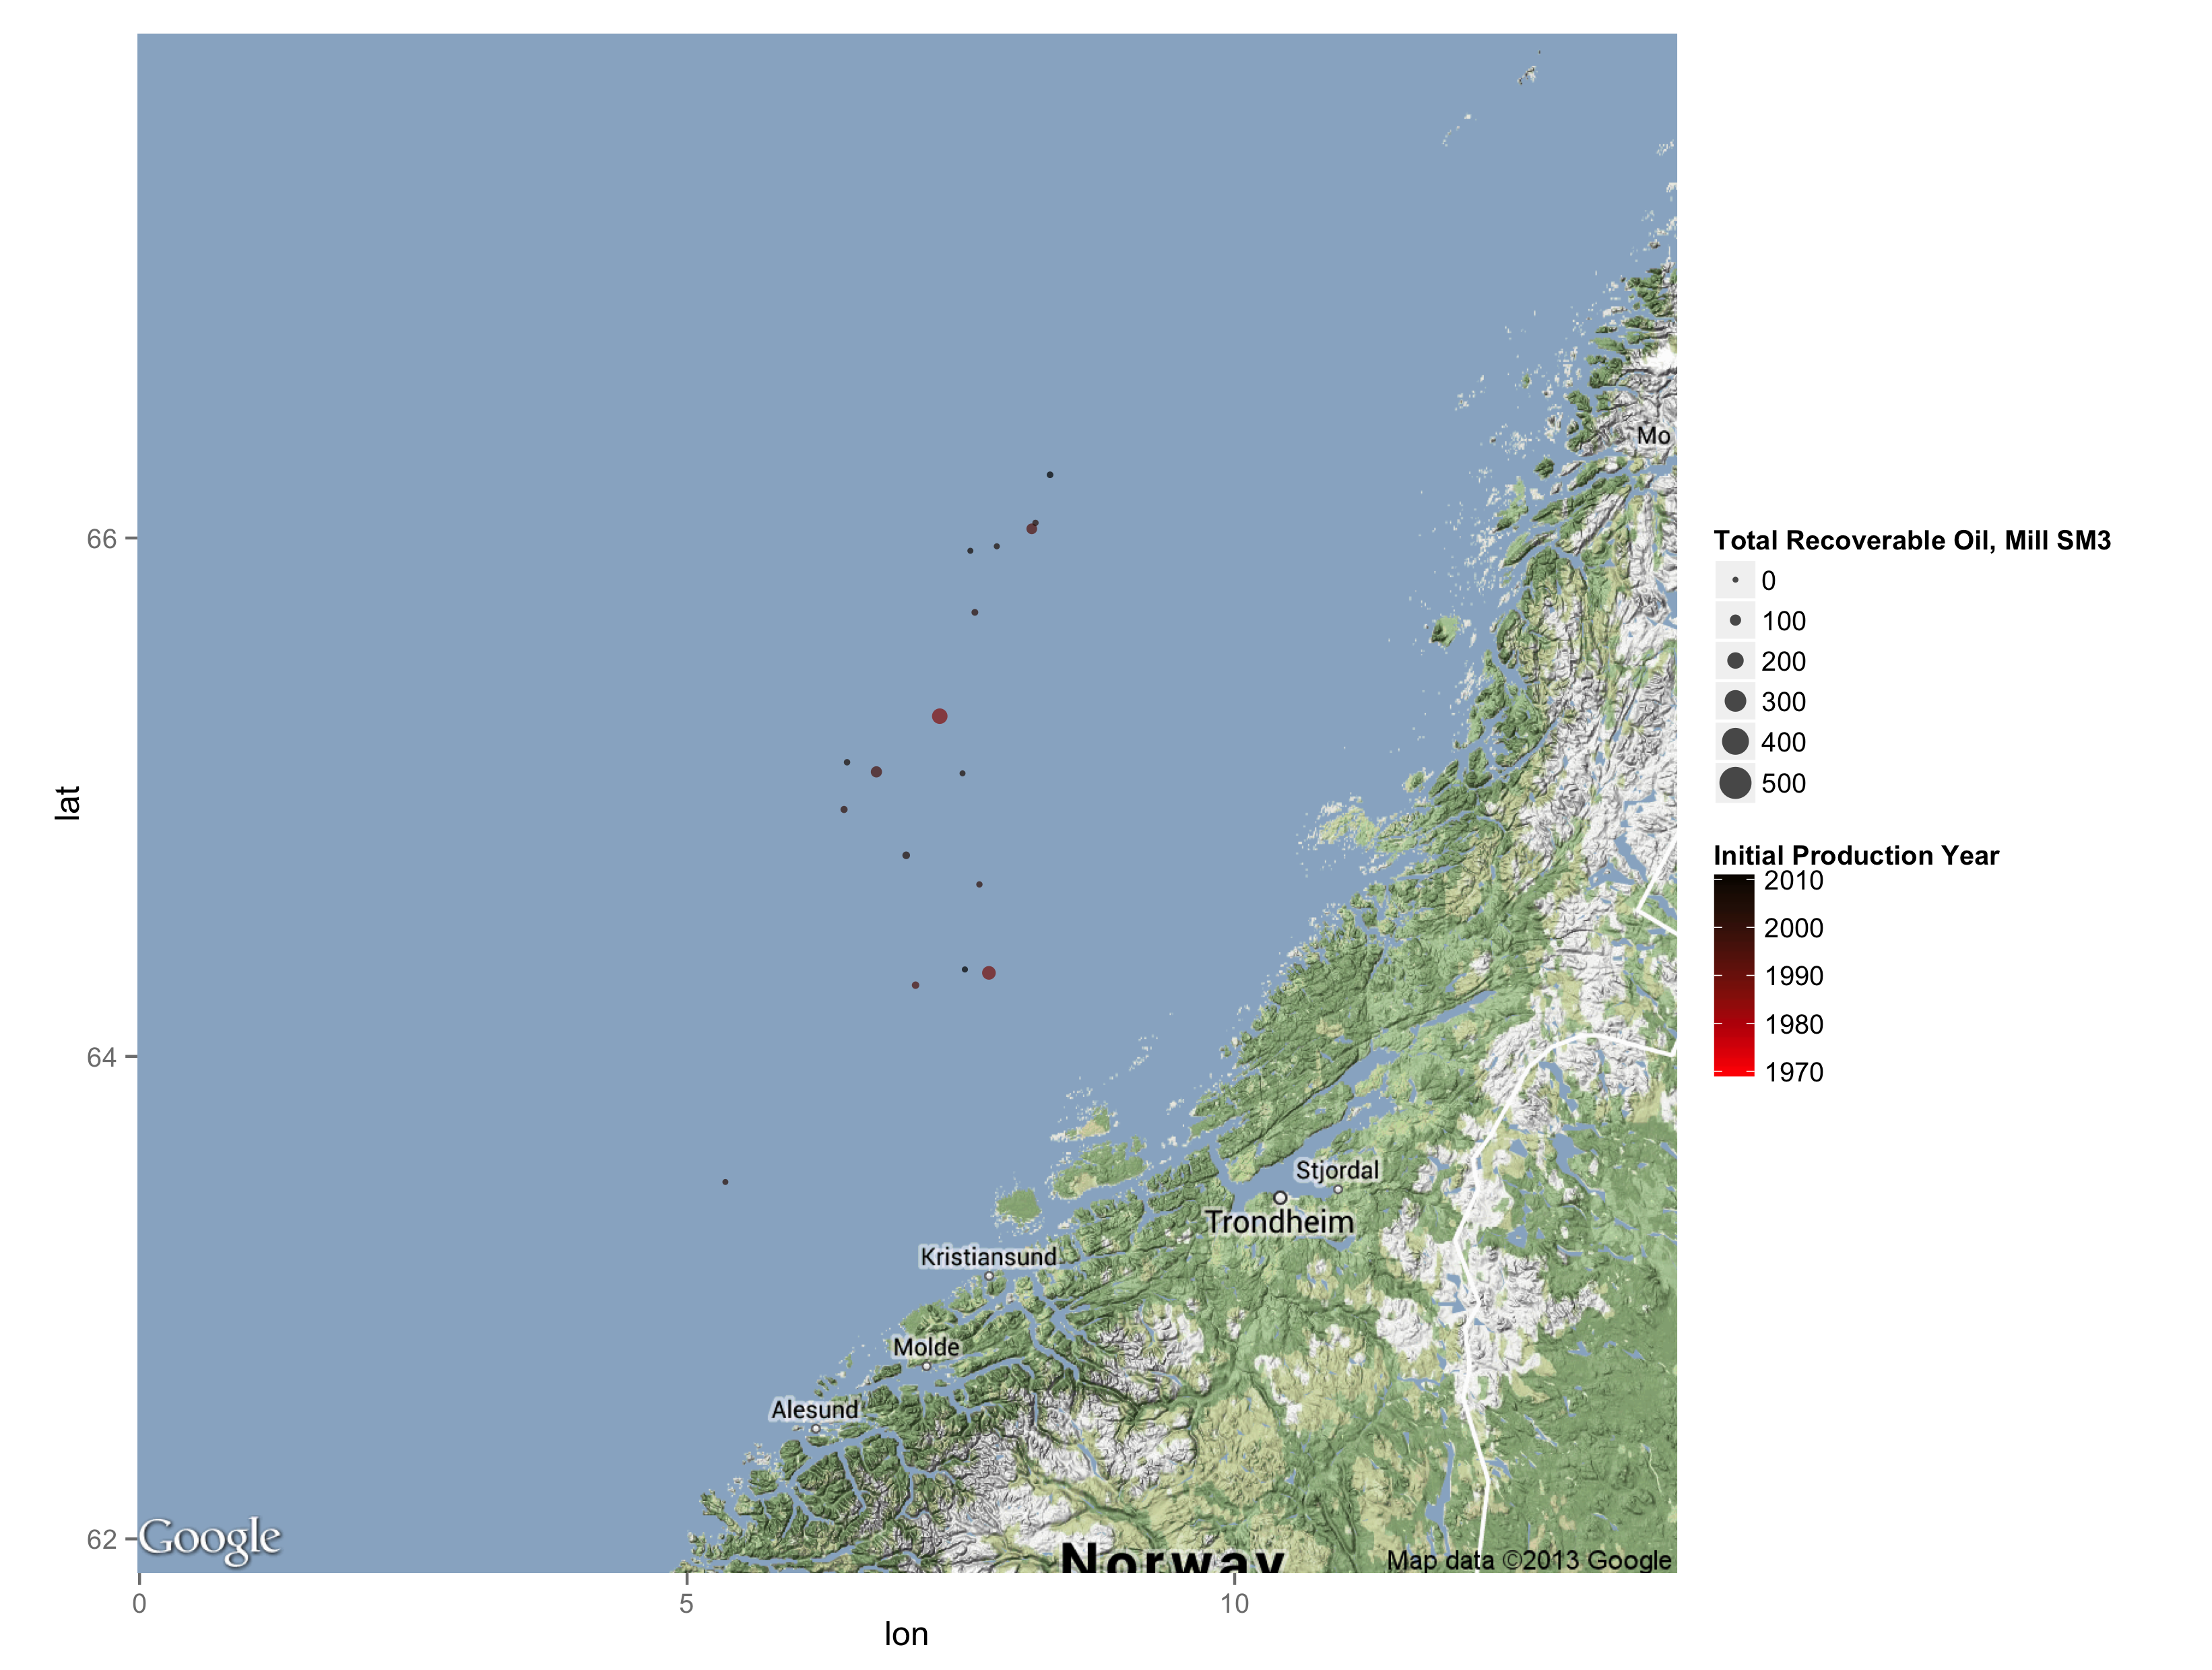
\includegraphics[width=.8\textwidth]{figures/norwegian_sea_reserves.png}
	\caption*{}
	\label{norwegian_sea_reserves}
	\end{figure}
\end{frame}


\begin{frame}[plain]

\begin{figure}
	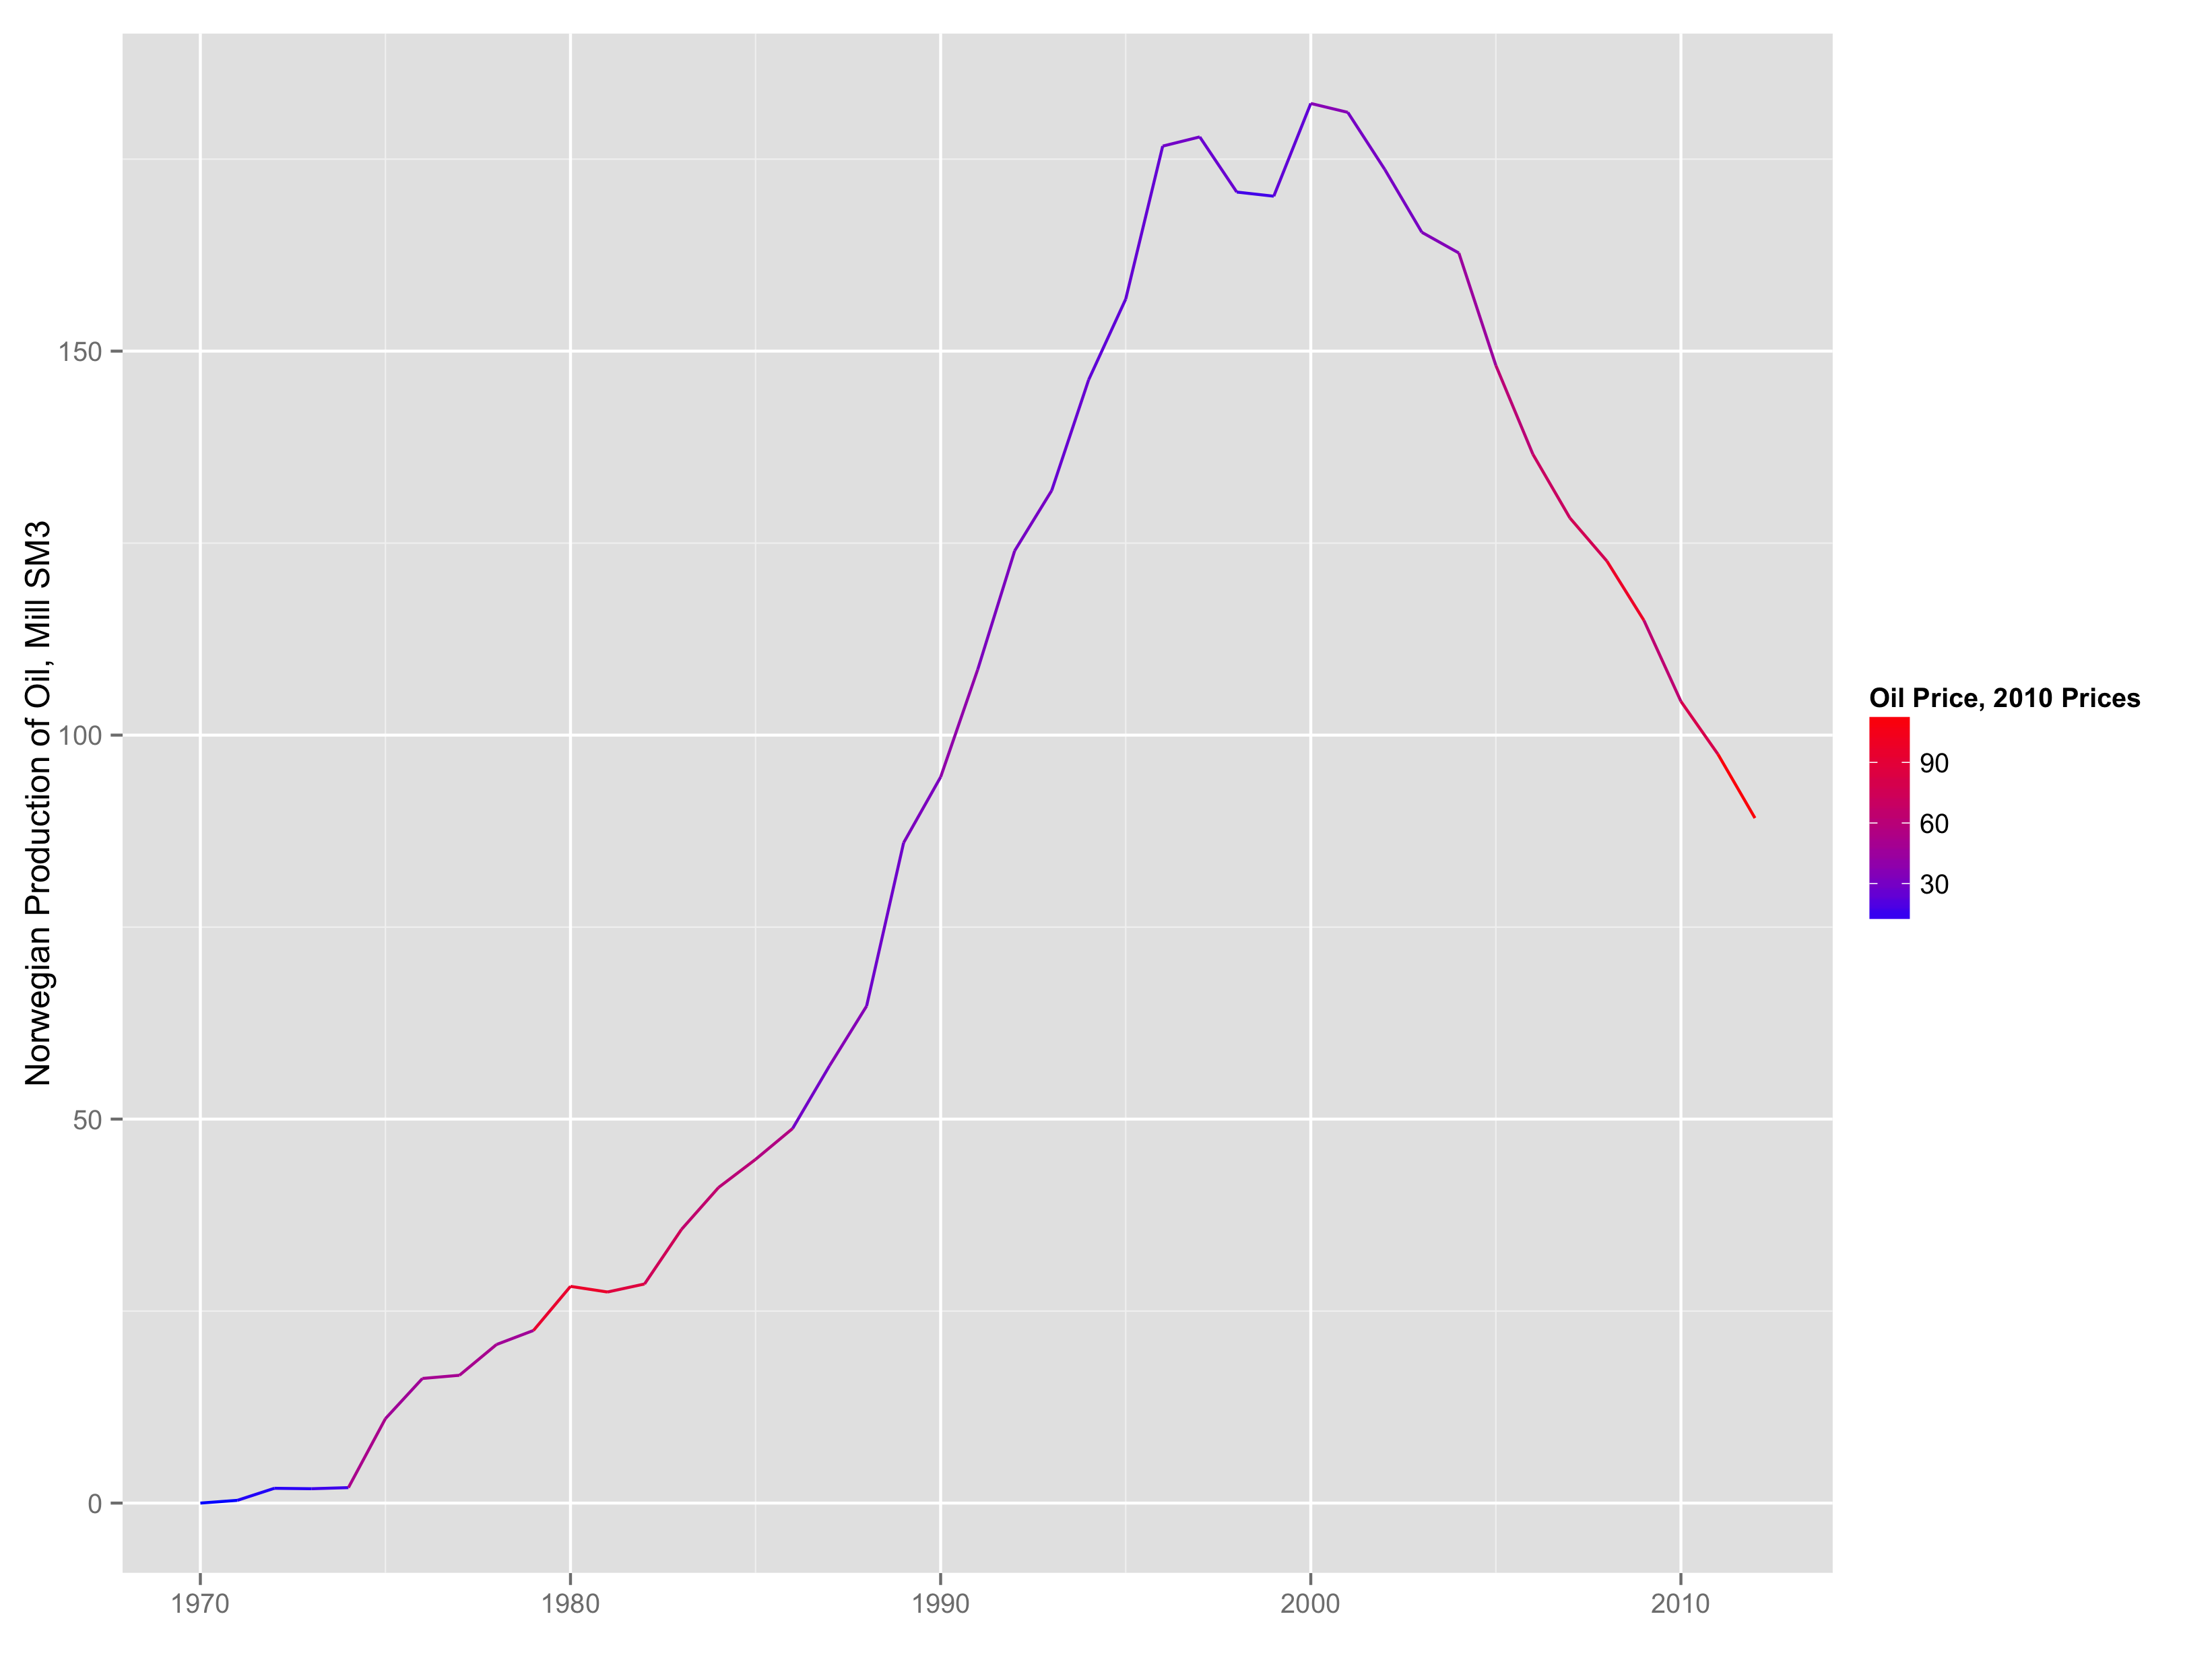
\includegraphics[width=.8\textwidth]{figures/oil_decline.png}
	\caption*{}
	\label{oil_decline}
\end{figure}

\end{frame}


\begin{frame}[plain]
	\begin{figure}
	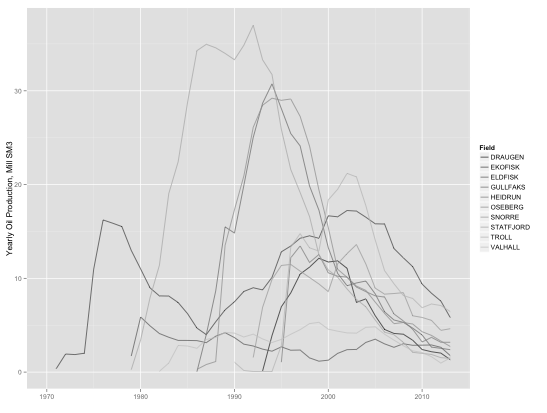
\includegraphics[width=.8\textwidth]{figures/top10_production.png}
	\caption*{}
	\label{top10_production}	
	\end{figure}
\end{frame}







\begin{frame}[plain]
	\begin{equation}
		\begin{split}
		 Log(Production_{i,t}) & = \alpha_0 + \alpha_1 time\_to\_peak_{i,t} + \alpha_2 time\_to\_peak_{i,t}^2 \\
		& \quad + \alpha_3 time\_to\_peak_{i,t}^3  + \alpha_4 peak\_to\_end_{i,t} + \alpha_5 peak\_to\_end_{i,t}^2 \\
		& \quad + \alpha_6 peak\_to\_end_{i,t}^3 + \gamma total\_recoverable\_oil_i \\
		& \quad + \beta_1 oil\_price + \beta_2 oil\_price\_l1 + ...+ \epsilon
		\end{split}
	\label{glm_eqn}
		\end{equation}
\end{frame}


\begin{frame}[plain]
	\begin{figure}
	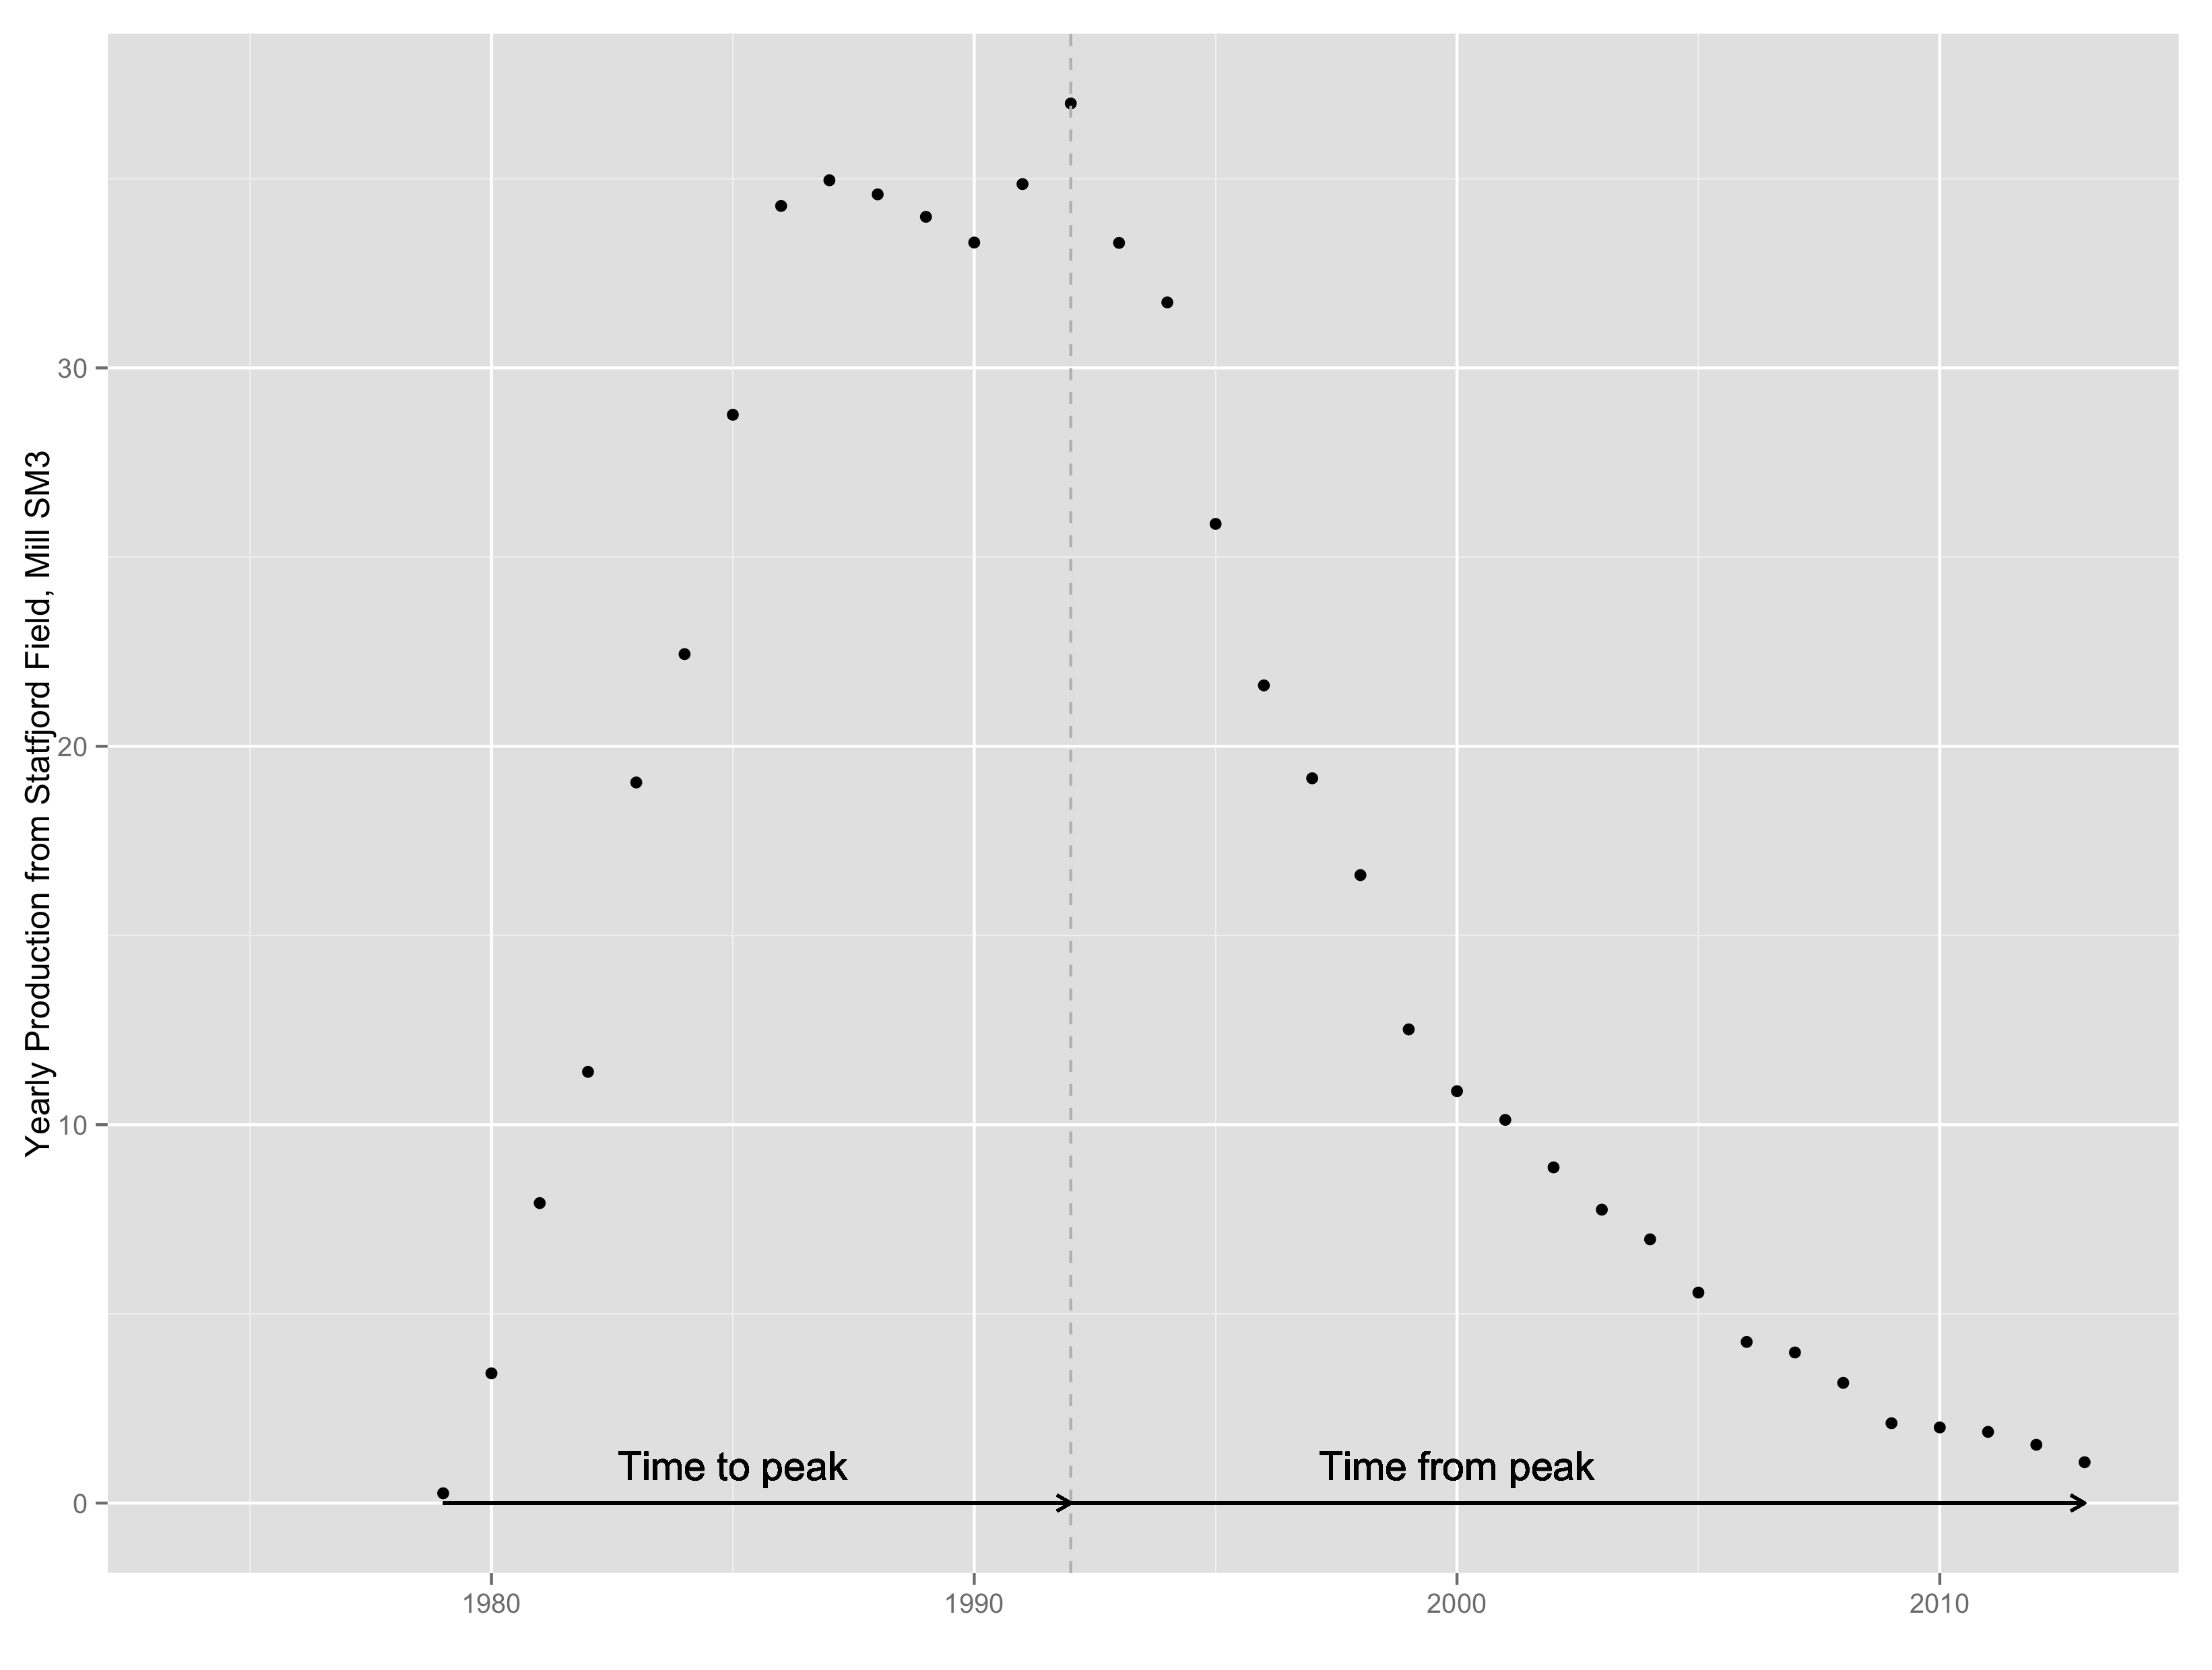
\includegraphics[width=.8\textwidth]{figures/statfjord_dem.png}
	\caption*{}
	\label{statfjord_dem}
	\end{figure}
\end{frame}


\begin{frame}[plain]
	\begin{figure}
	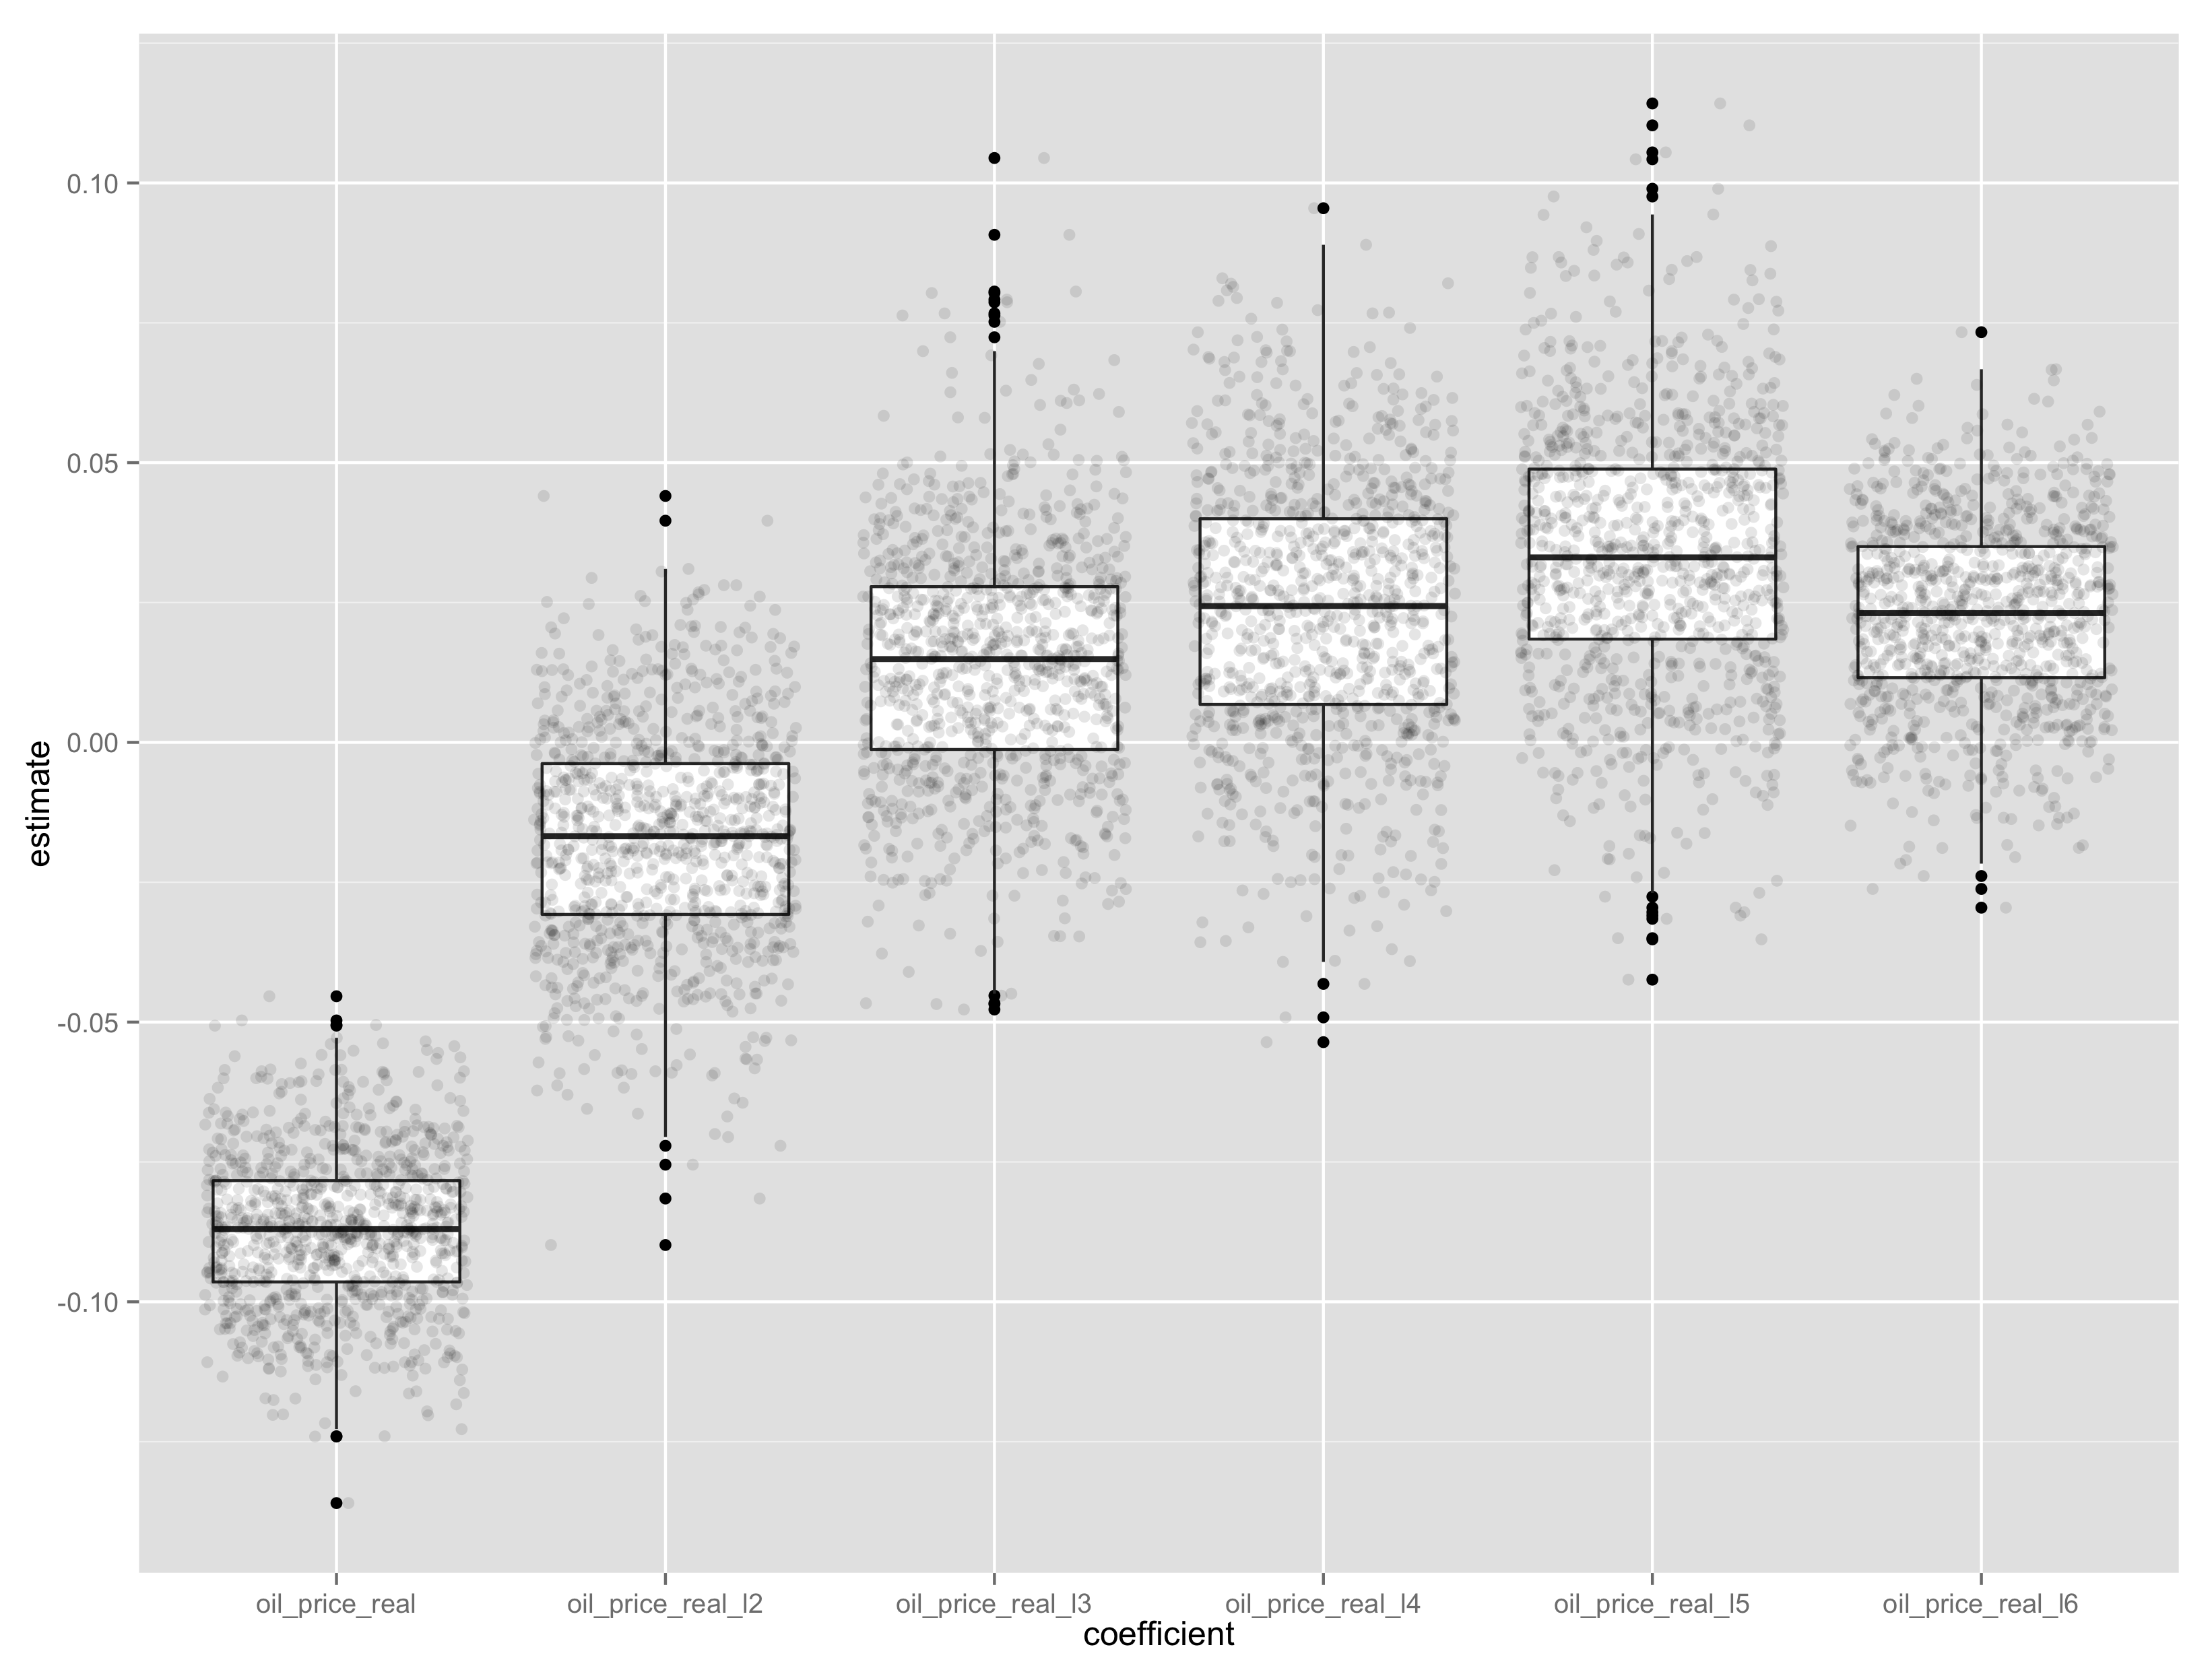
\includegraphics[width=.8\textwidth]{figures/glm_dirty_box.png}
	\caption*{}
	\label{glm_dirty_box}
	\end{figure}
\end{frame}


\begin{frame}[plain]
	\begin{equation}
	Production_{t}=f(time) + \epsilon
		\label{simp_eqn}
	\end{equation}
\end{frame}


\begin{frame}[plain]
	\begin{figure}
		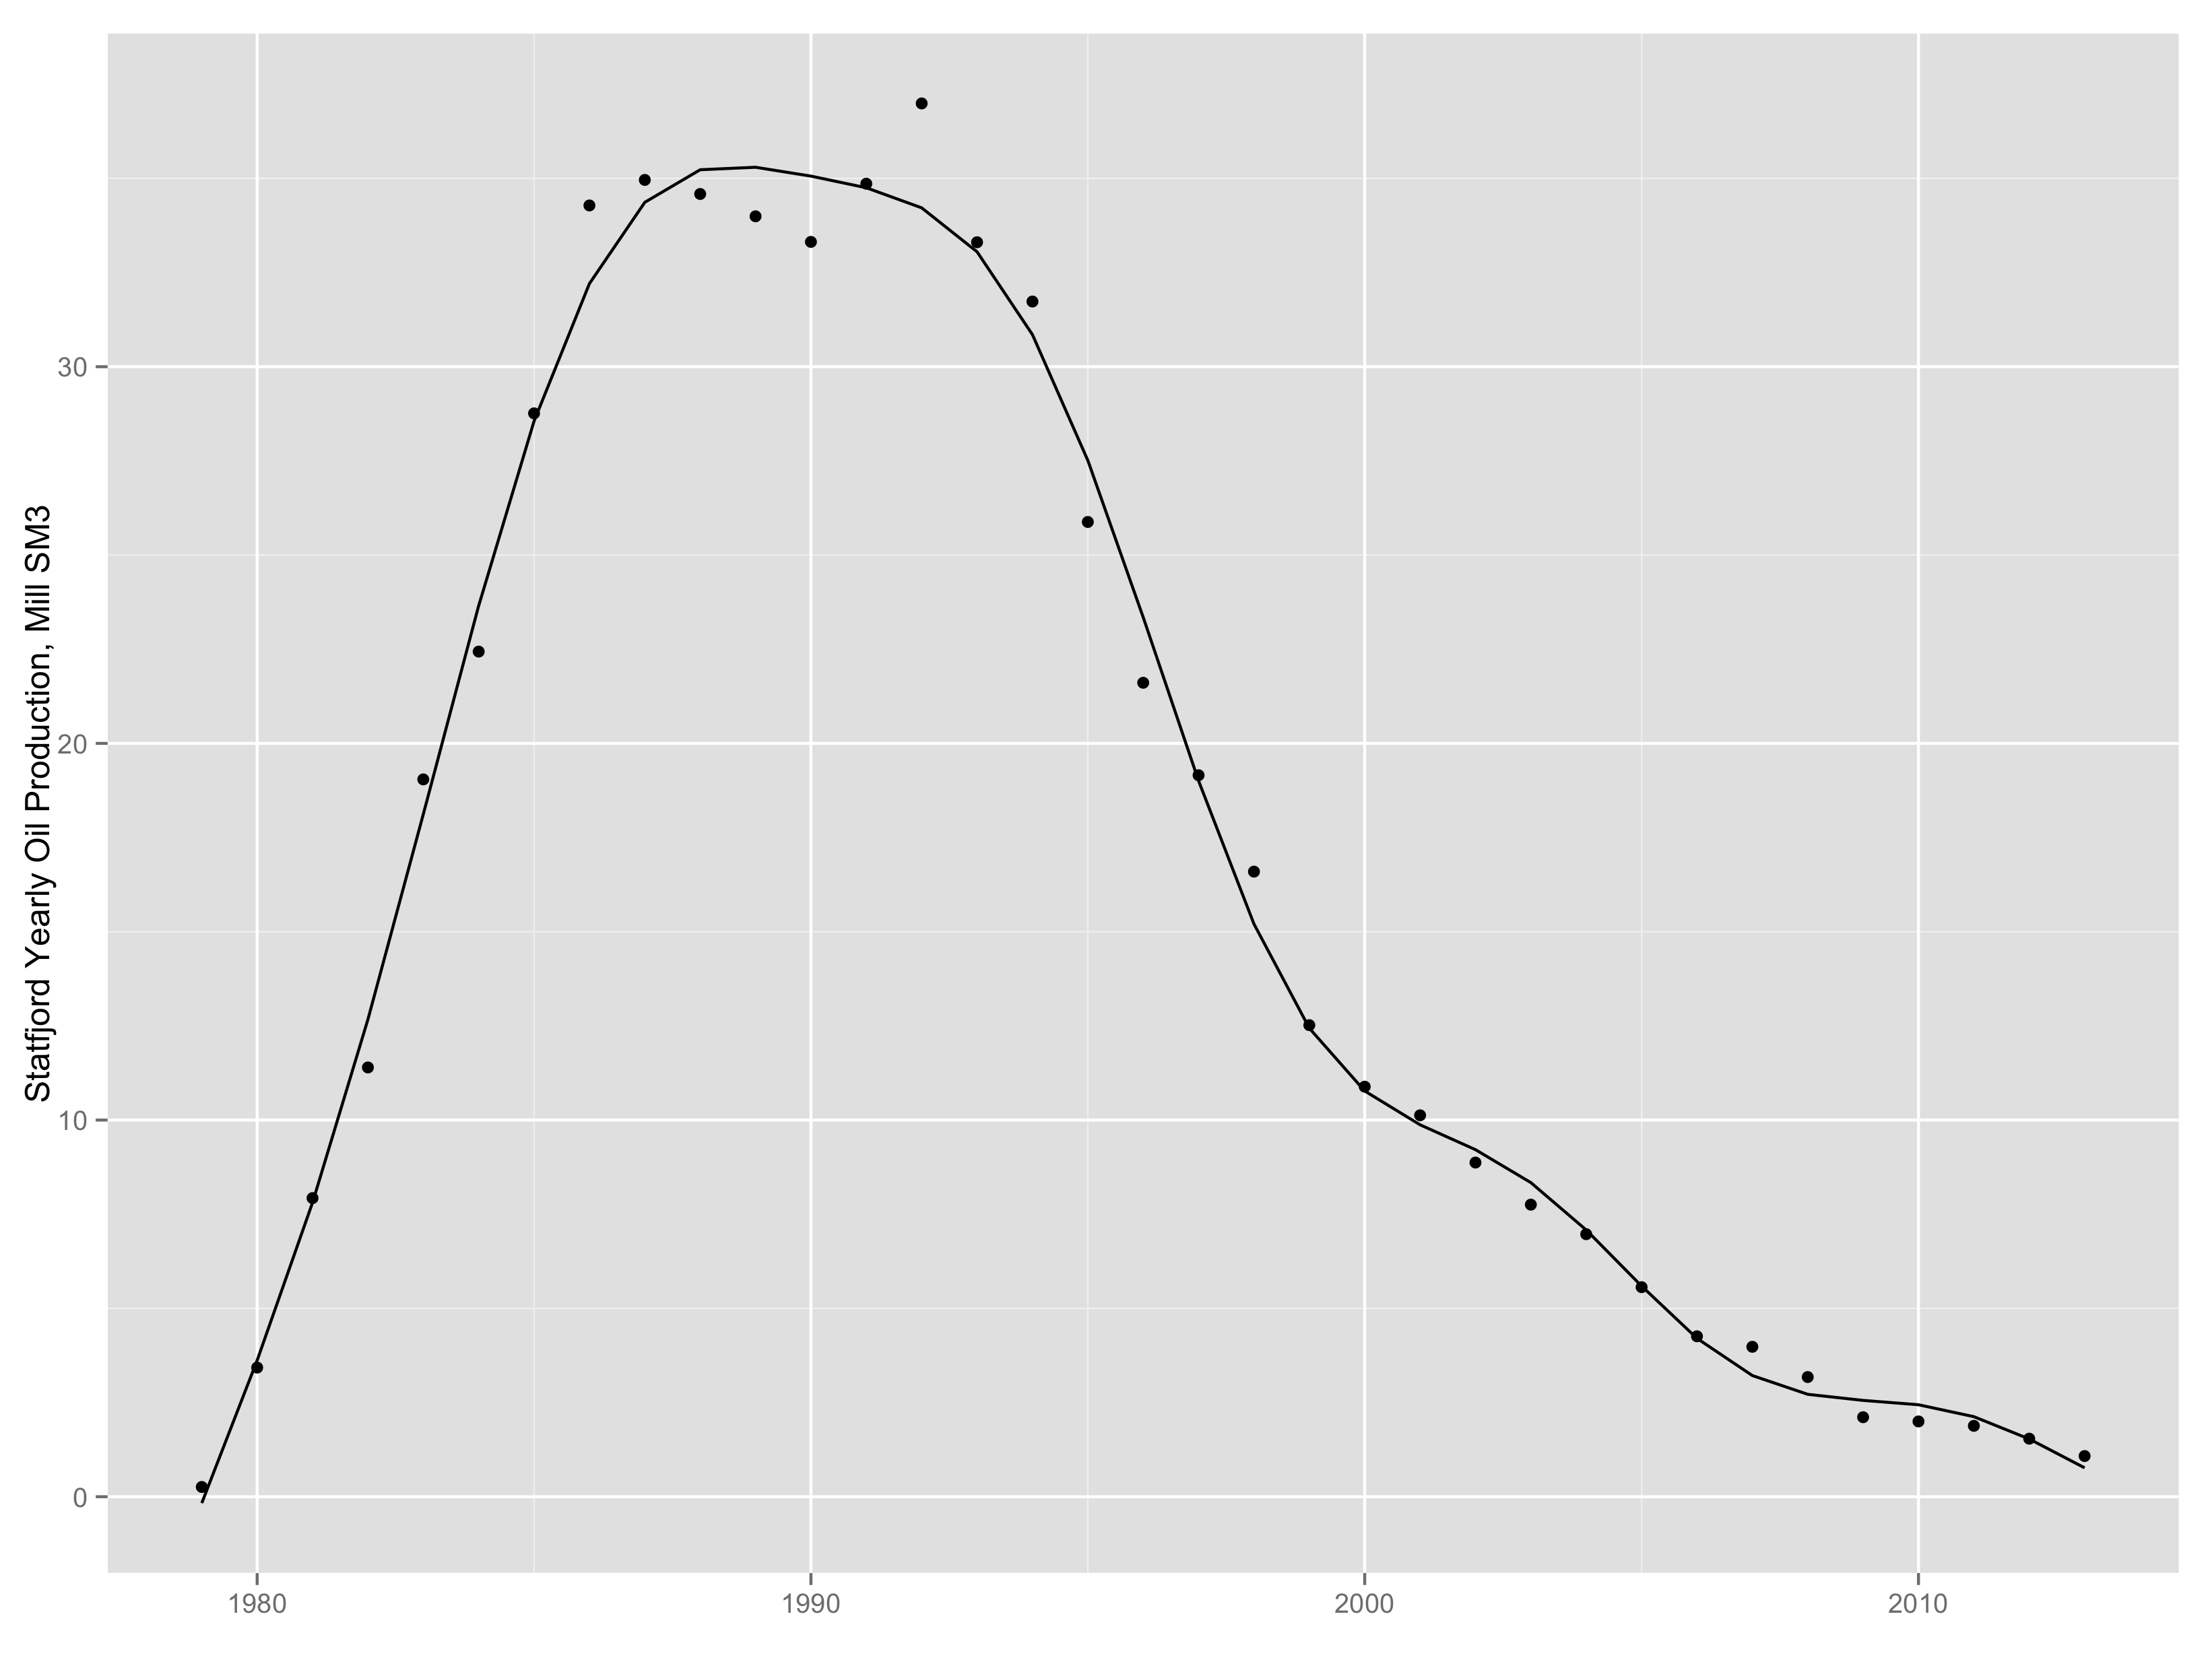
\includegraphics[width=.8\textwidth]{figures/statfjord_gam.png}
		\caption*{}
		\label{statfjord_gam}
	\end{figure}
\end{frame}


\begin{frame}[plain]

	\begin{equation}
	\begin{split}
		Log(Production_{i,t})&=f(time\_to\_peak_{i,t}, total\_recoverable\_oil_i) \\
		& \quad + f(peak\_to\_end_{i,t}, total\_recoverable\_oil_i) \\
		& \quad + \beta_1 oil\_price + \beta_2 oil\_price\_l1 + ... +  \epsilon
	\end{split}
	\label{gam_price_eqn}
	\end{equation}

\end{frame}



\begin{frame}[plain]
	Thin Plate (Regression) Splines (Duchon 1977)
	\begin{equation}
	y_i = g(x_1, x_2)
	\end{equation}

	\begin{equation}
	\min \|\boldsymbol{y-f}\|^2 + \lambda J_{md}(f)
	\end{equation}

	\begin{equation}
	J_{22}{f}= \diffp[2]{f}{x_1}^2 + \diffp[2]{f}{{x_1}{x_2}} + \diffp[2]{f}{x_2}^2dx_1 dx_2
	\end{equation}
\end{frame}

\begin{frame}[plain]
	\begin{figure}
		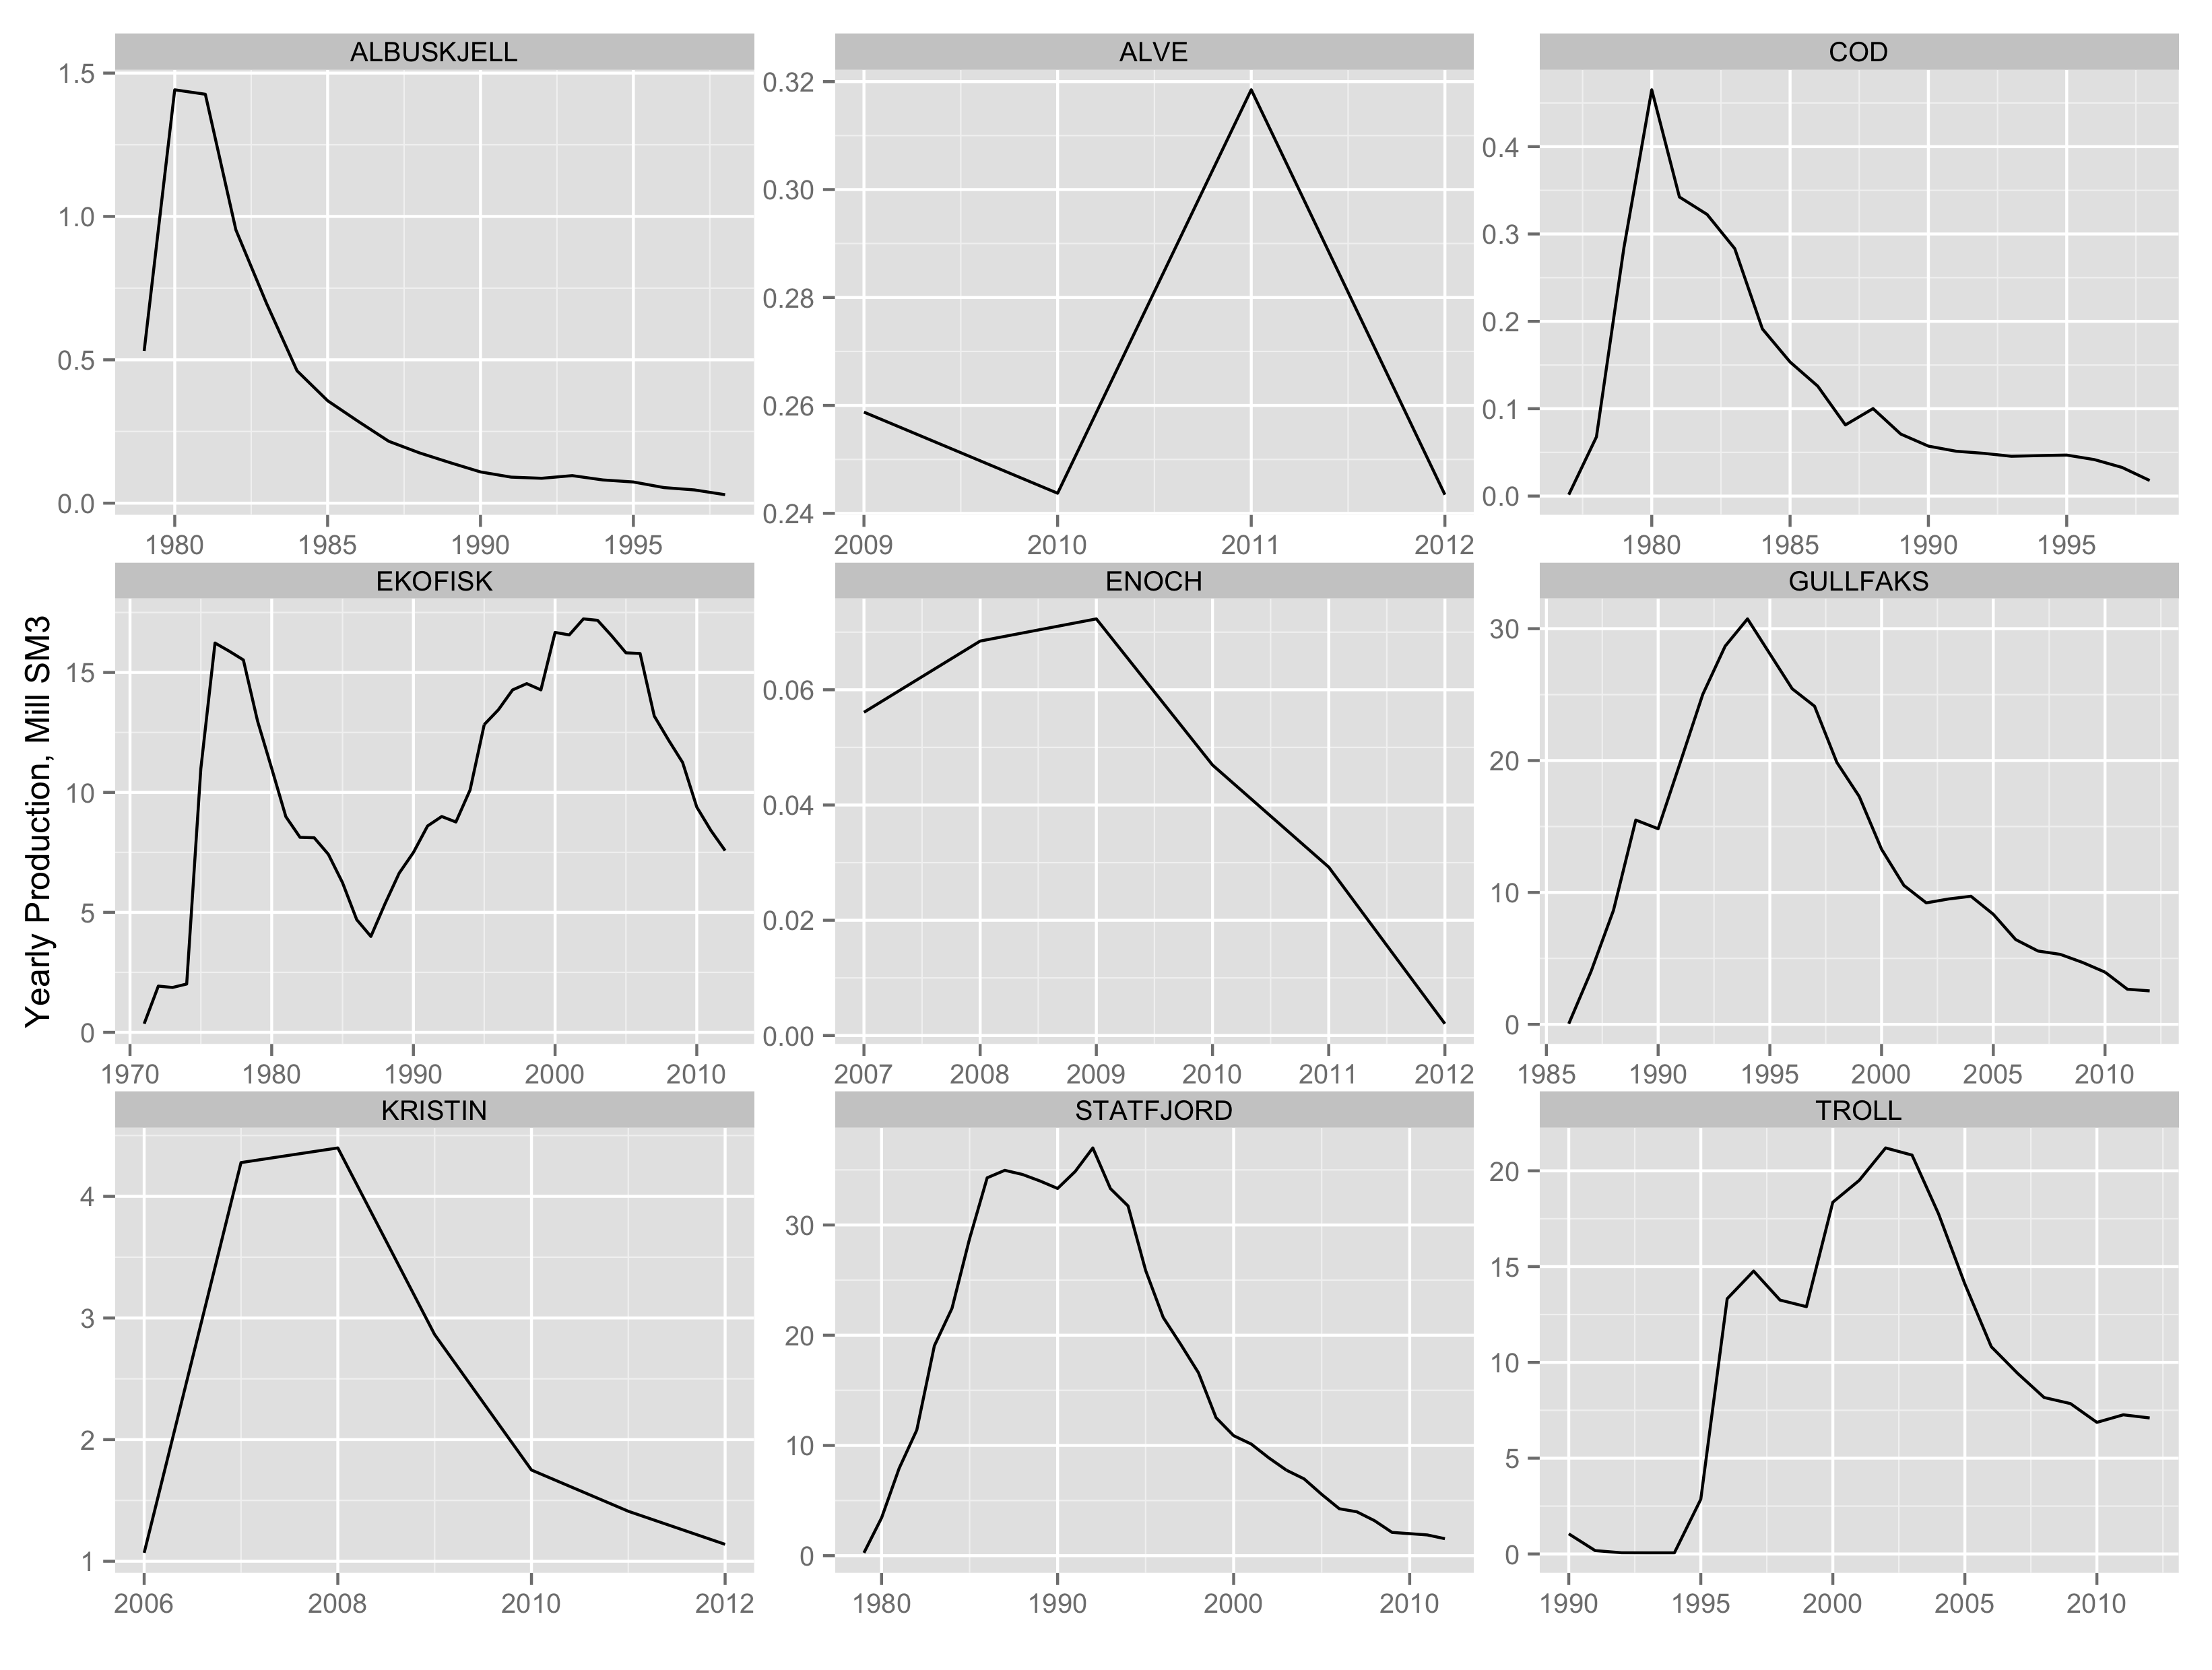
\includegraphics[width=.8\textwidth]{figures/field_inspection.png}
		\caption*{}
		\label{field_inspection}
	\end{figure}
\end{frame}


\begin{frame}[plain]
	\begin{figure}
		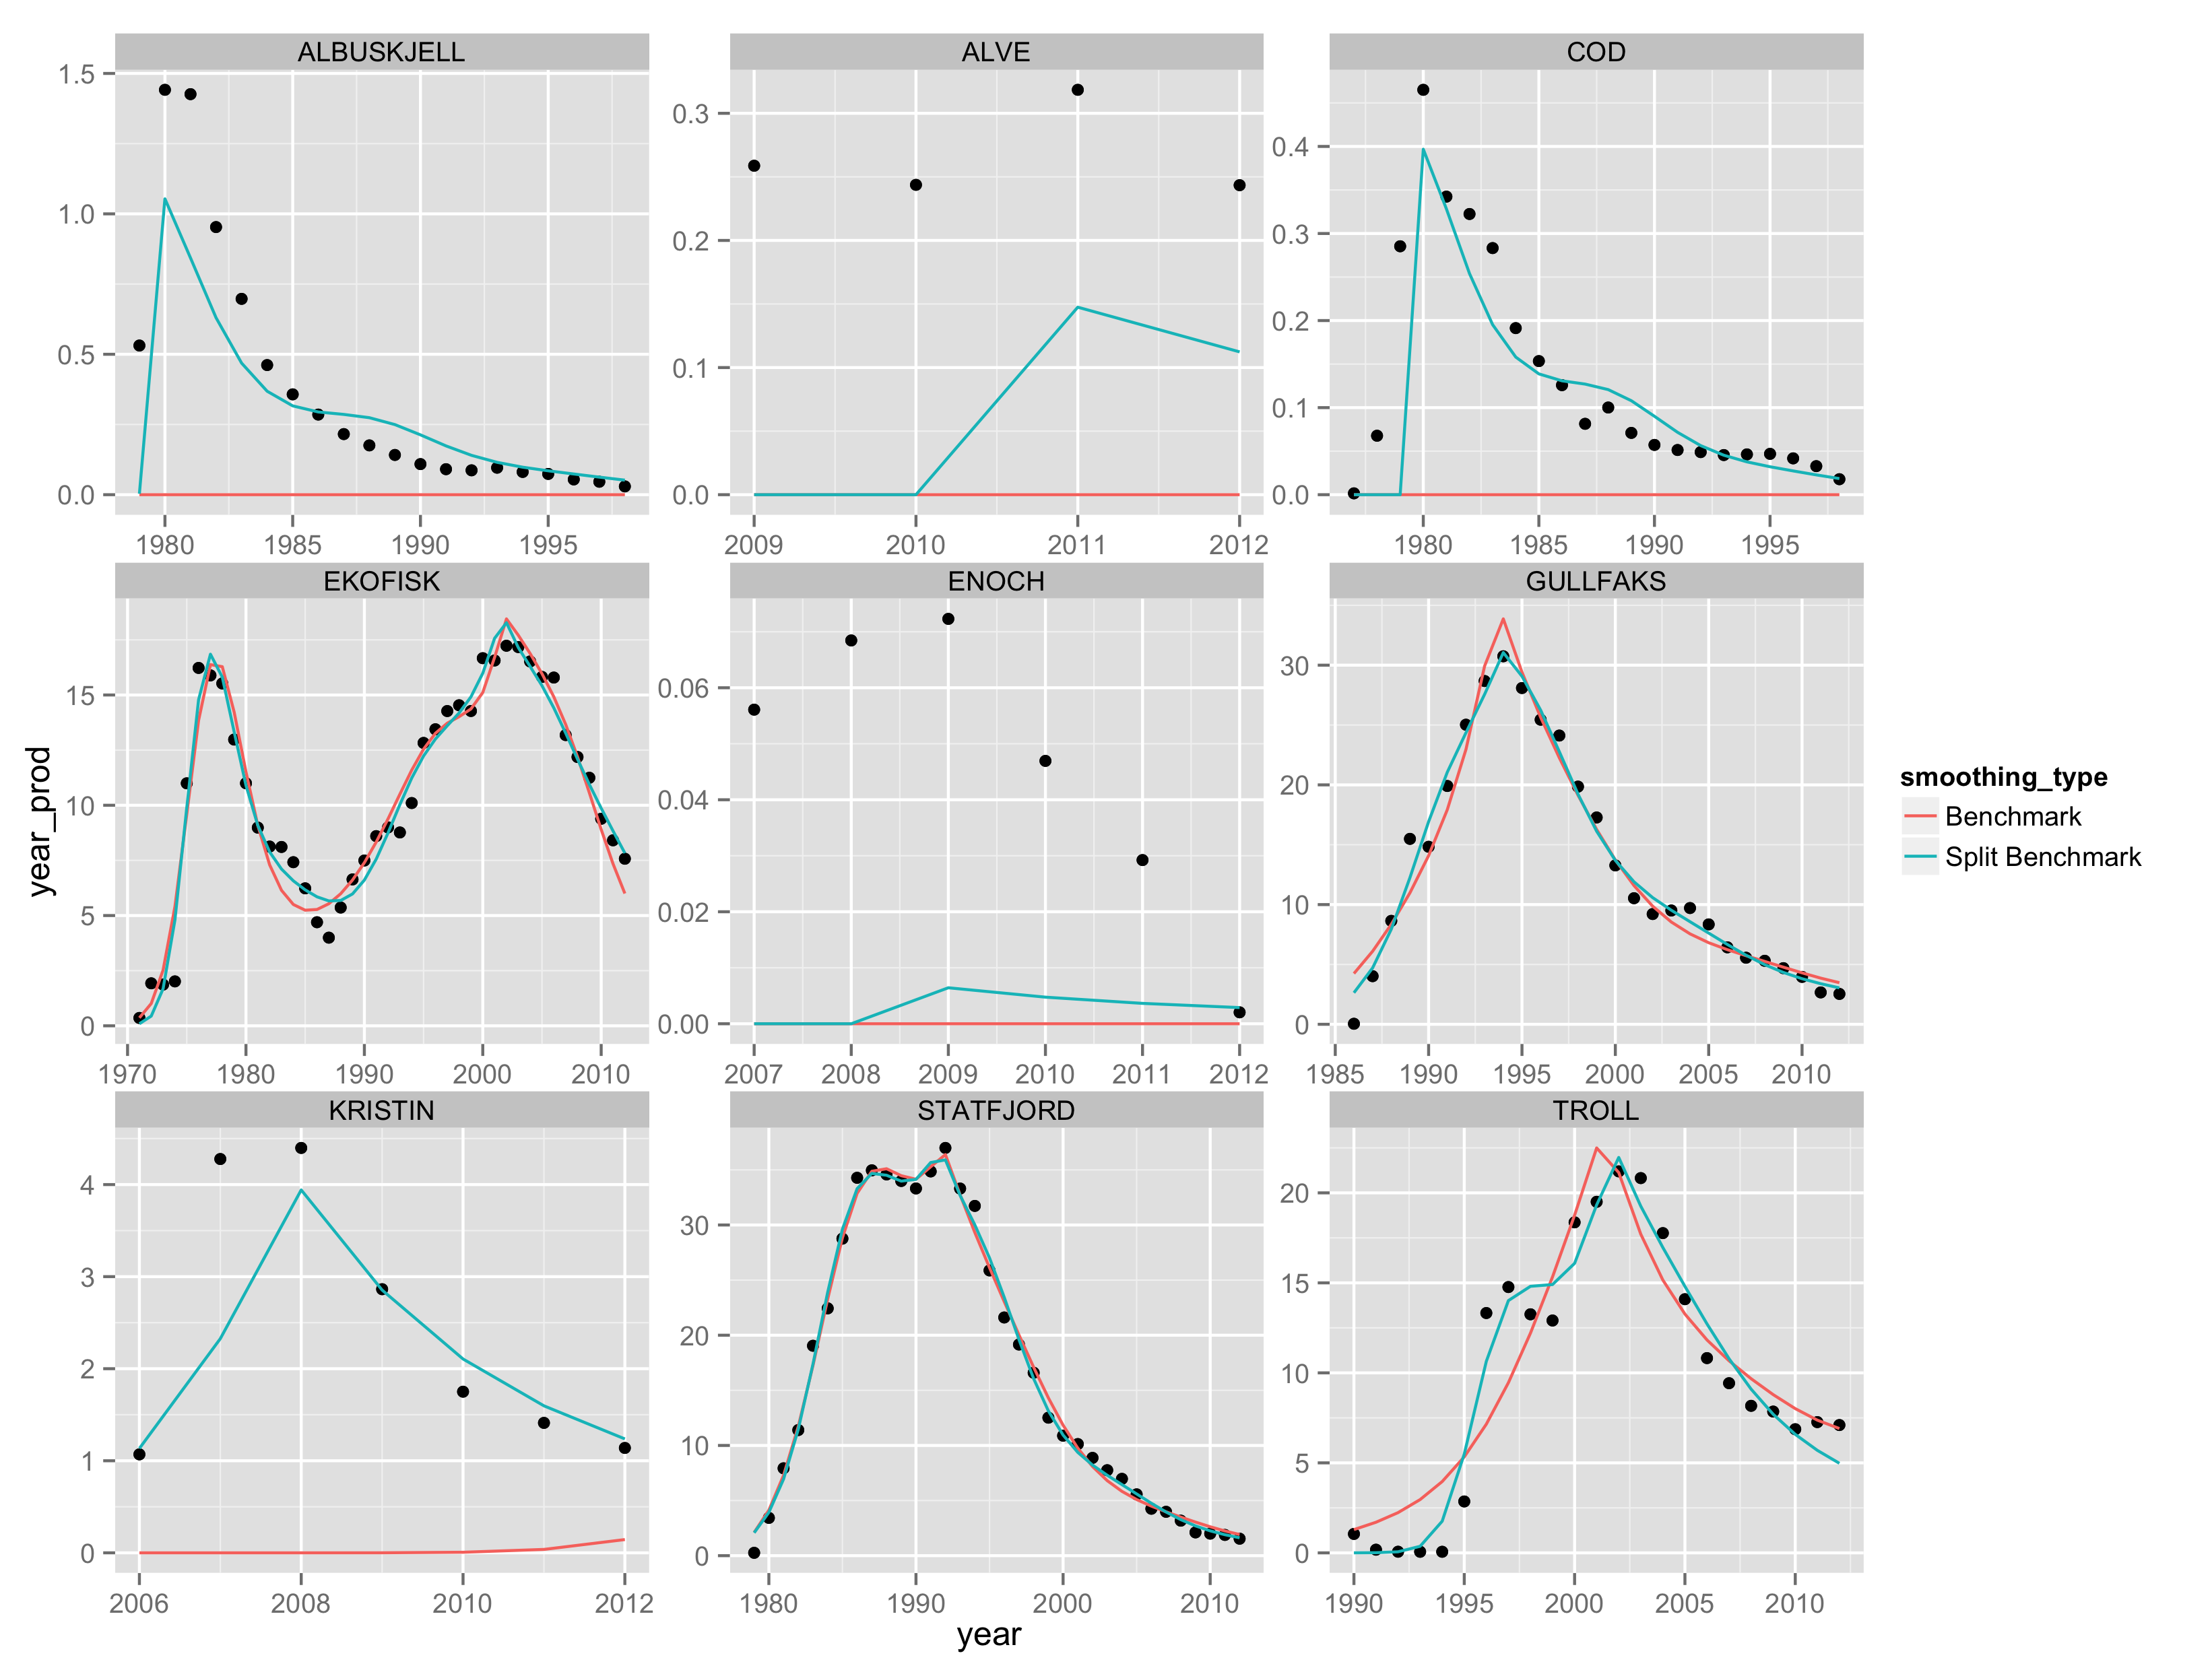
\includegraphics[width=.8\textwidth]{figures/bench_vs_split.png}
		\caption*{}
		\label{bench_vs_split}
	\end{figure}
\end{frame}


\begin{frame}[plain]
	\begin{figure}
		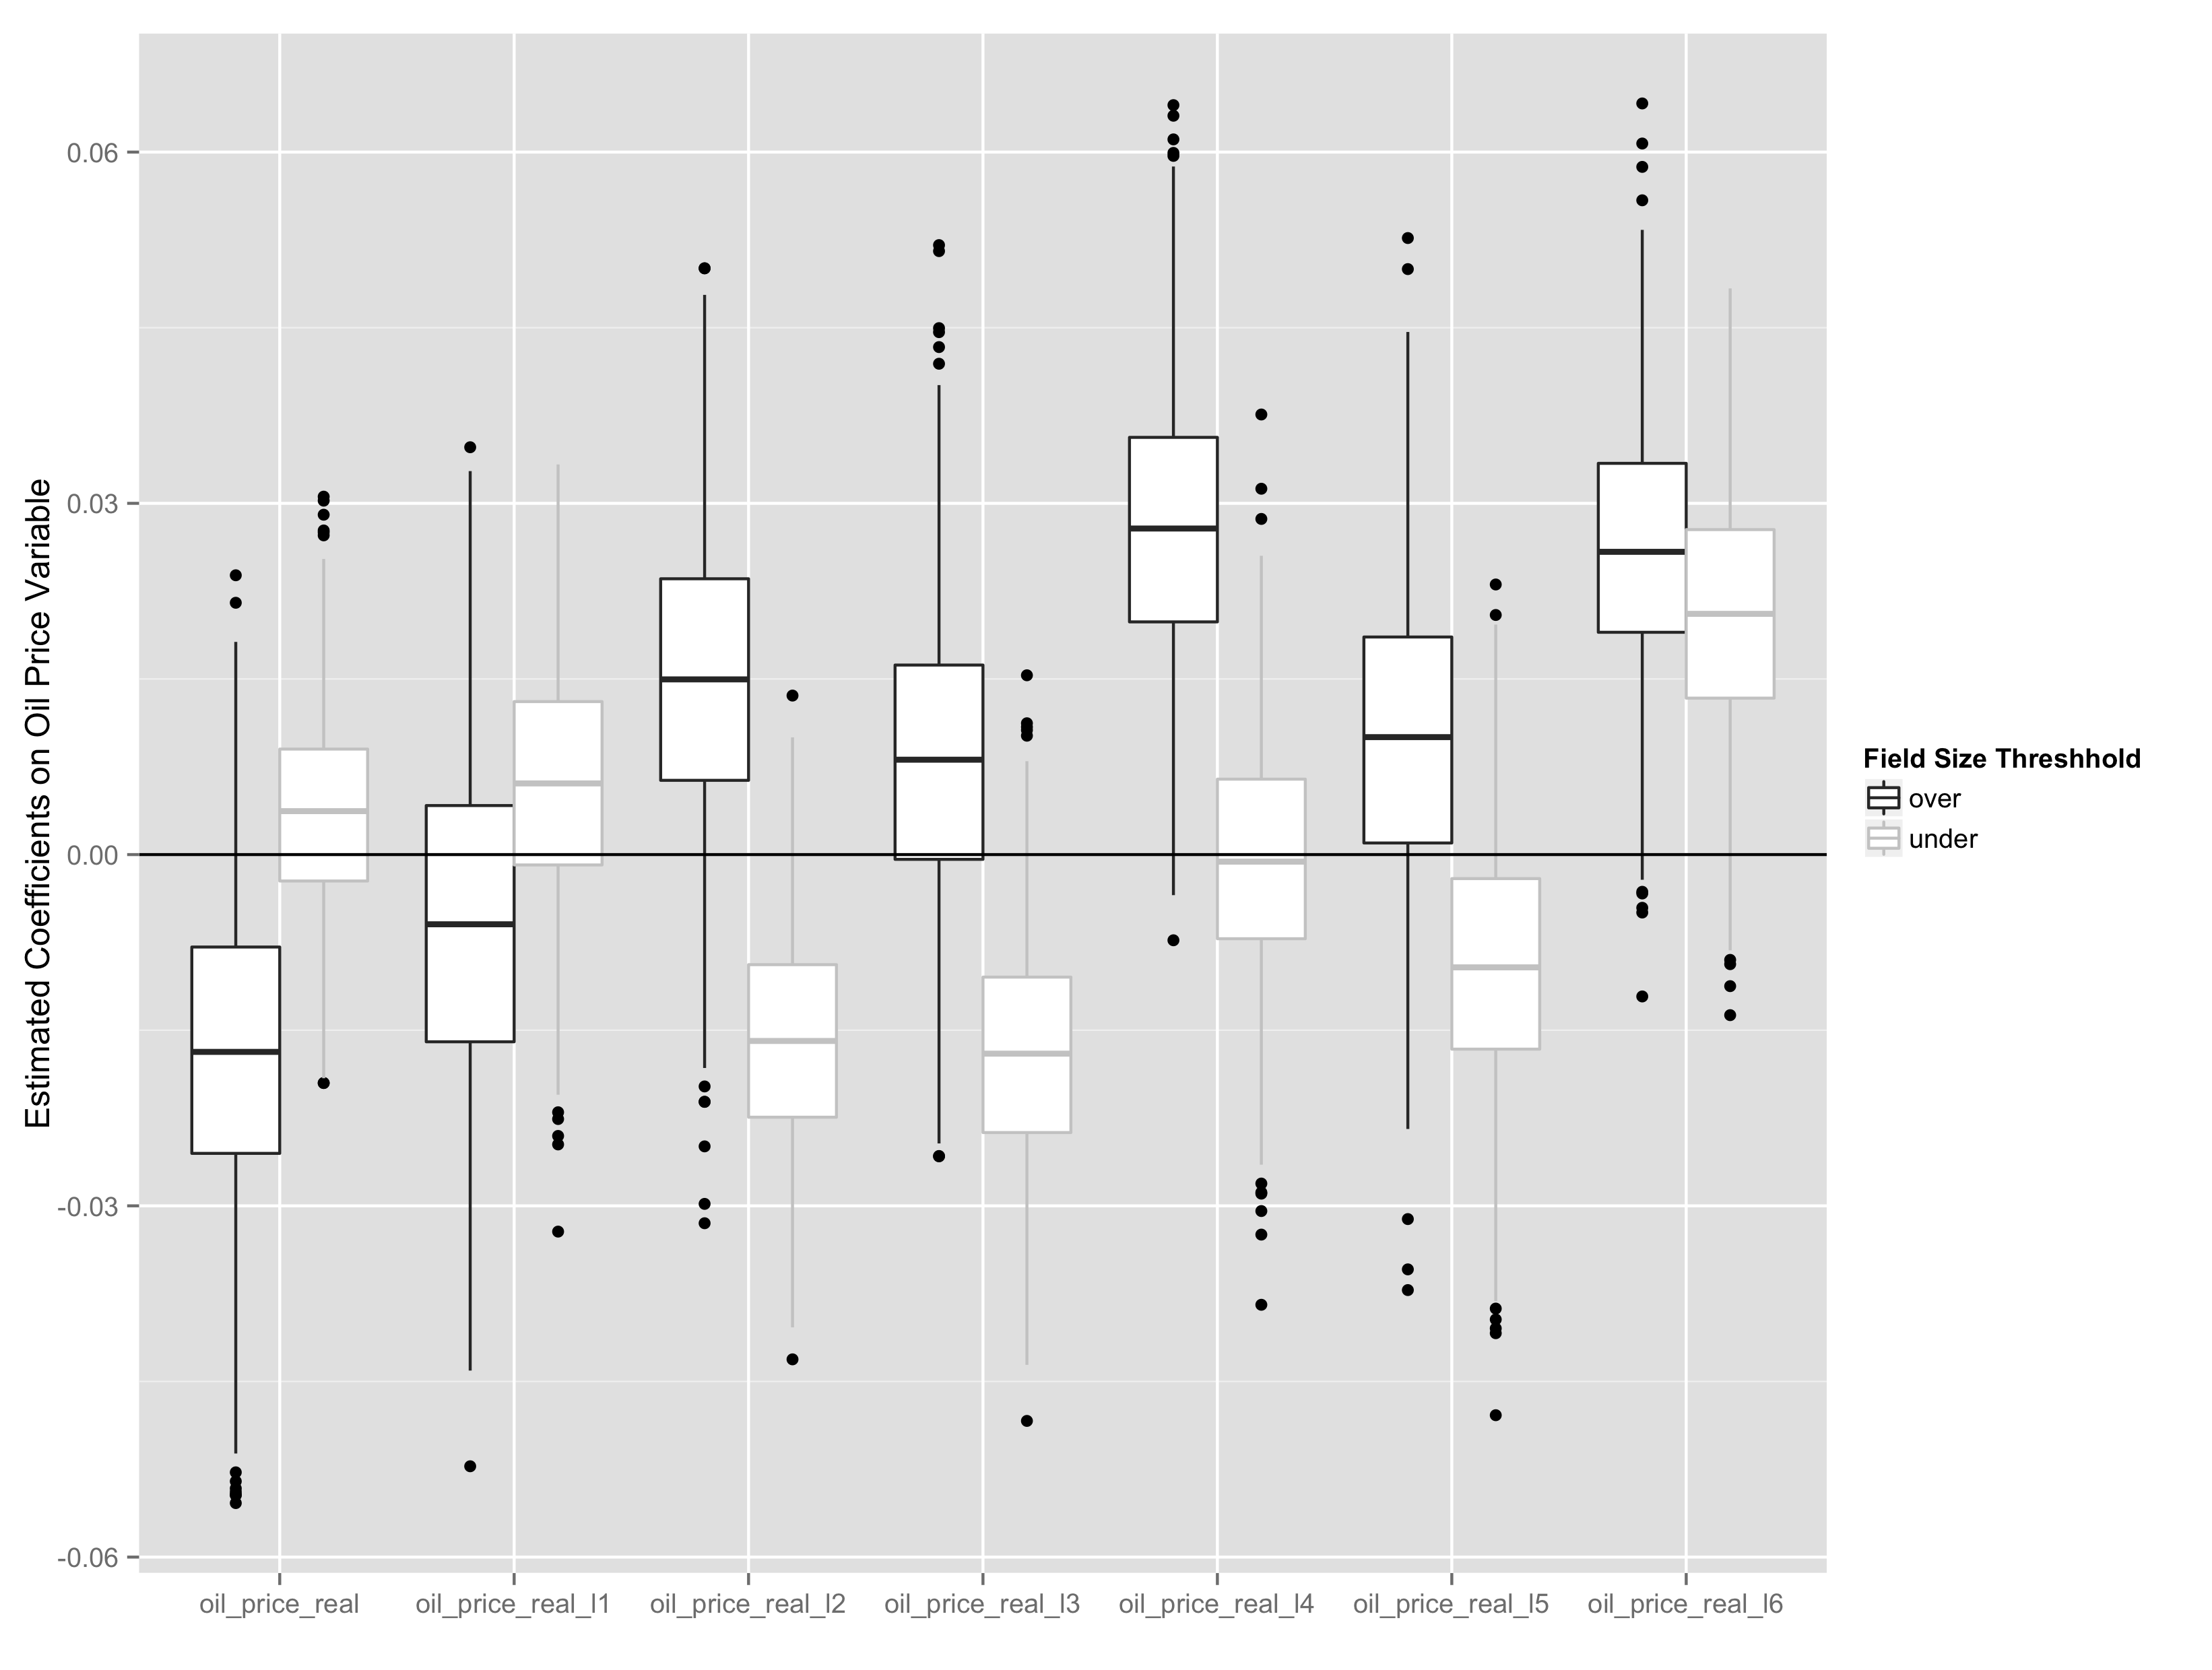
\includegraphics[width=.8\textwidth]{figures/gam_price_dirty_box.png}
		\caption*{}
		\label{gam_price_dirty_box}
	\end{figure}
\end{frame}


\begin{frame}[plain]
	\begin{equation}
	\begin{split}
		Log(Investment_{i,t})&=f(time\_to\_peak_{i,t}, total\_recoverable\_oil_i) \\
		& \quad + f(peak\_to\_end_{i,t}, total\_recoverable\_oil_i) \\
		& \quad + \alpha oil_production_{i,t} \\
		& \quad + \beta_1 oil\_price + \beta_2 oil\_price\_l1 + ... +  \epsilon
	\end{split}
	\label{gam_invest_eqn}
	\end{equation}
\end{frame}


\begin{frame}[plain]
	\begin{figure}
		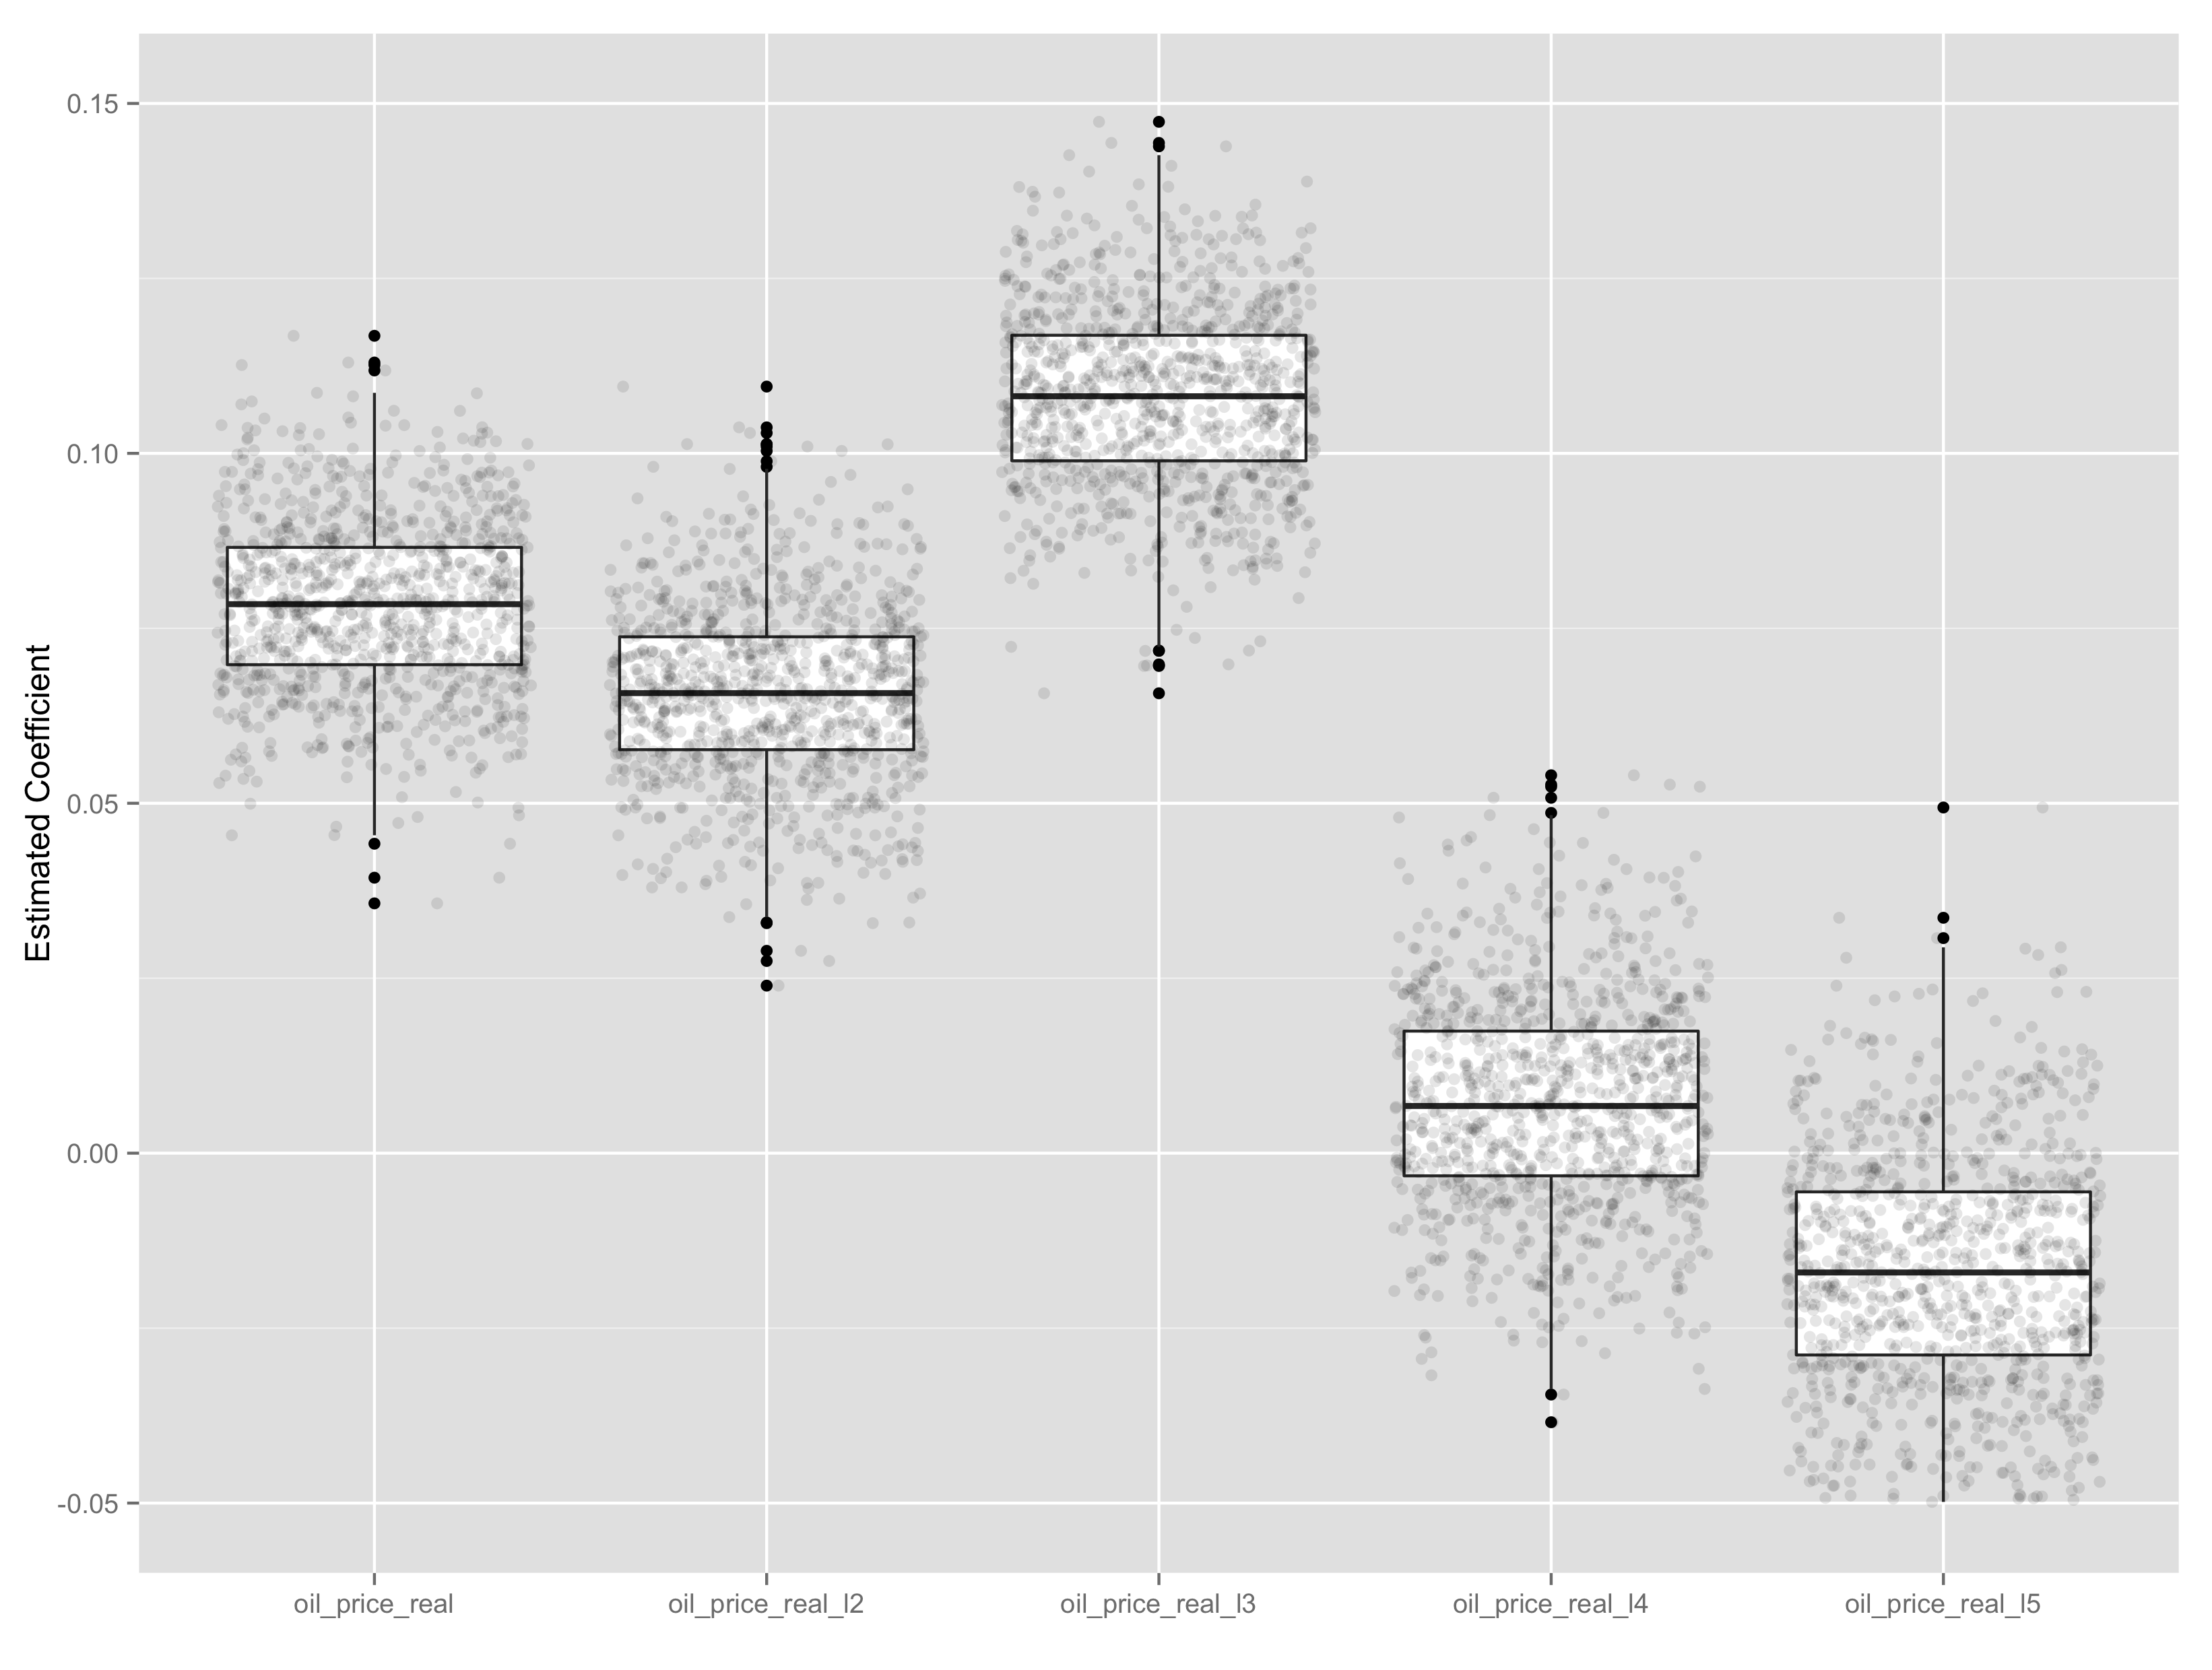
\includegraphics[width=.8\textwidth]{figures/gam_price_invest_box.png}
		\caption*{}
		\label{gam_price_invest_box}
	\end{figure}
\end{frame}

\begin{frame}[plain]

	\begin{figure}
		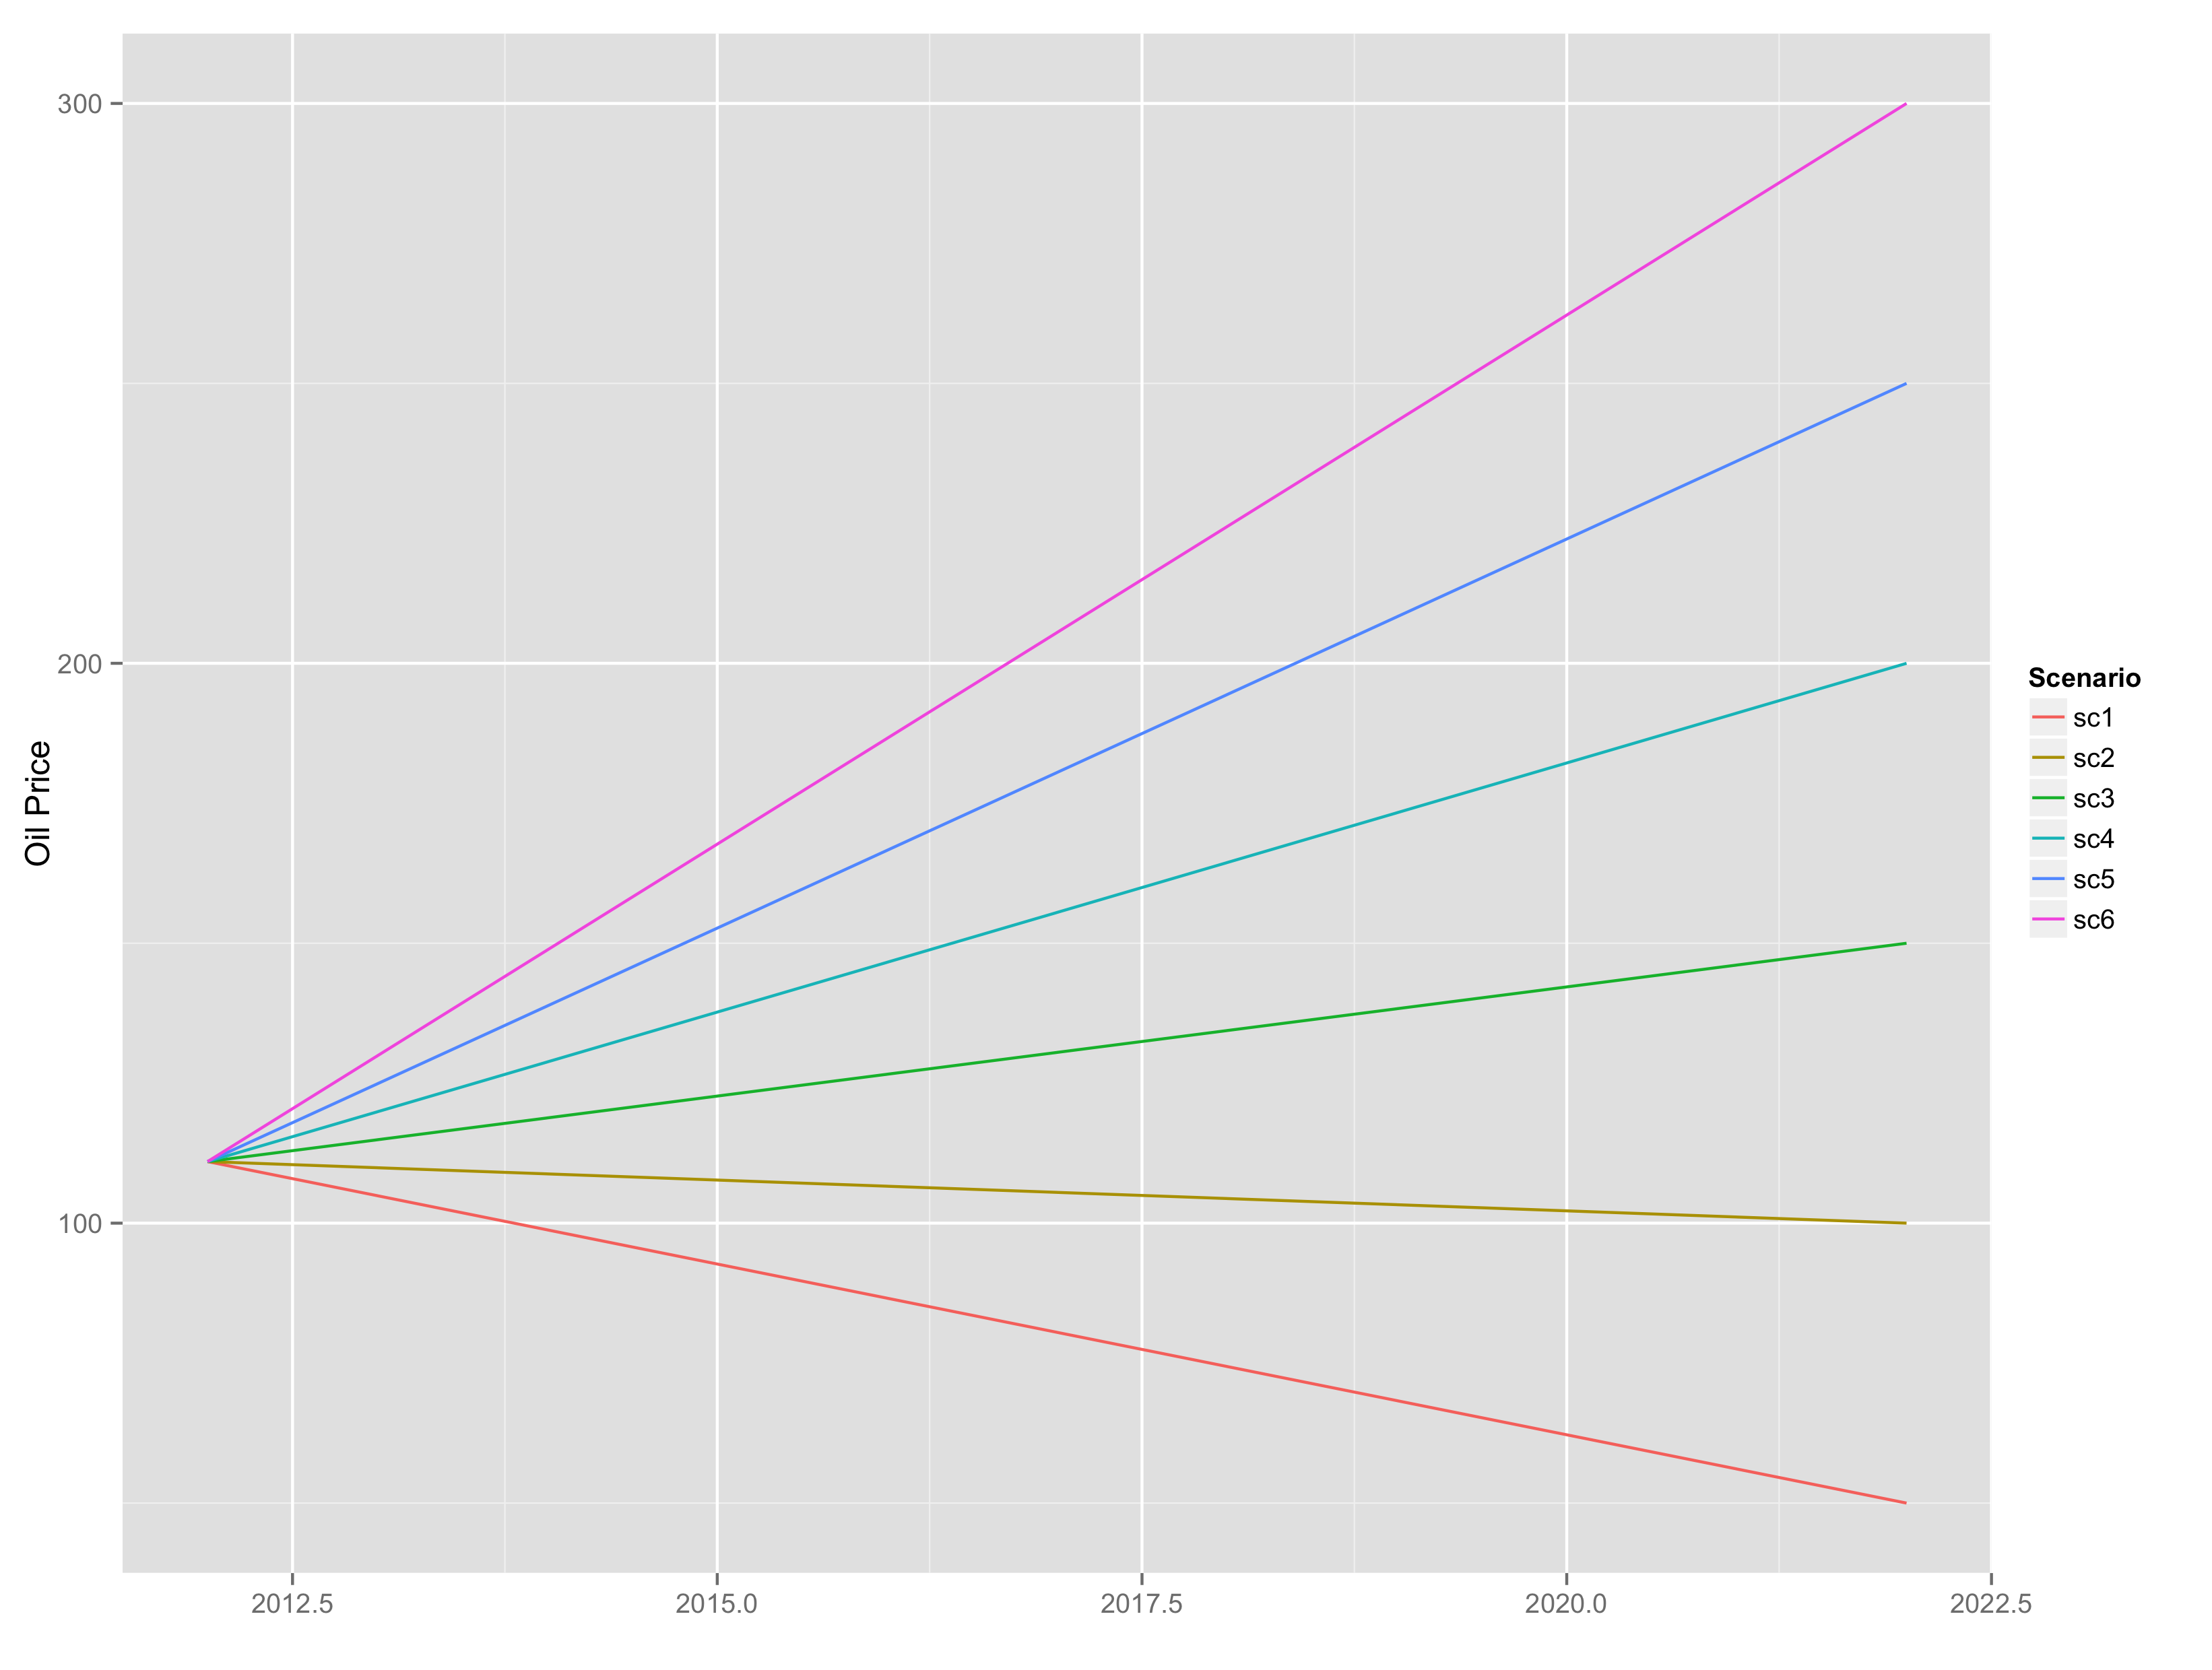
\includegraphics[width=.8\textwidth]{figures/price_scenario.png}
		\caption*{}
		\label{price_scenario}
\end{figure}
\end{frame}

\begin{frame}[plain]
	\begin{figure}
		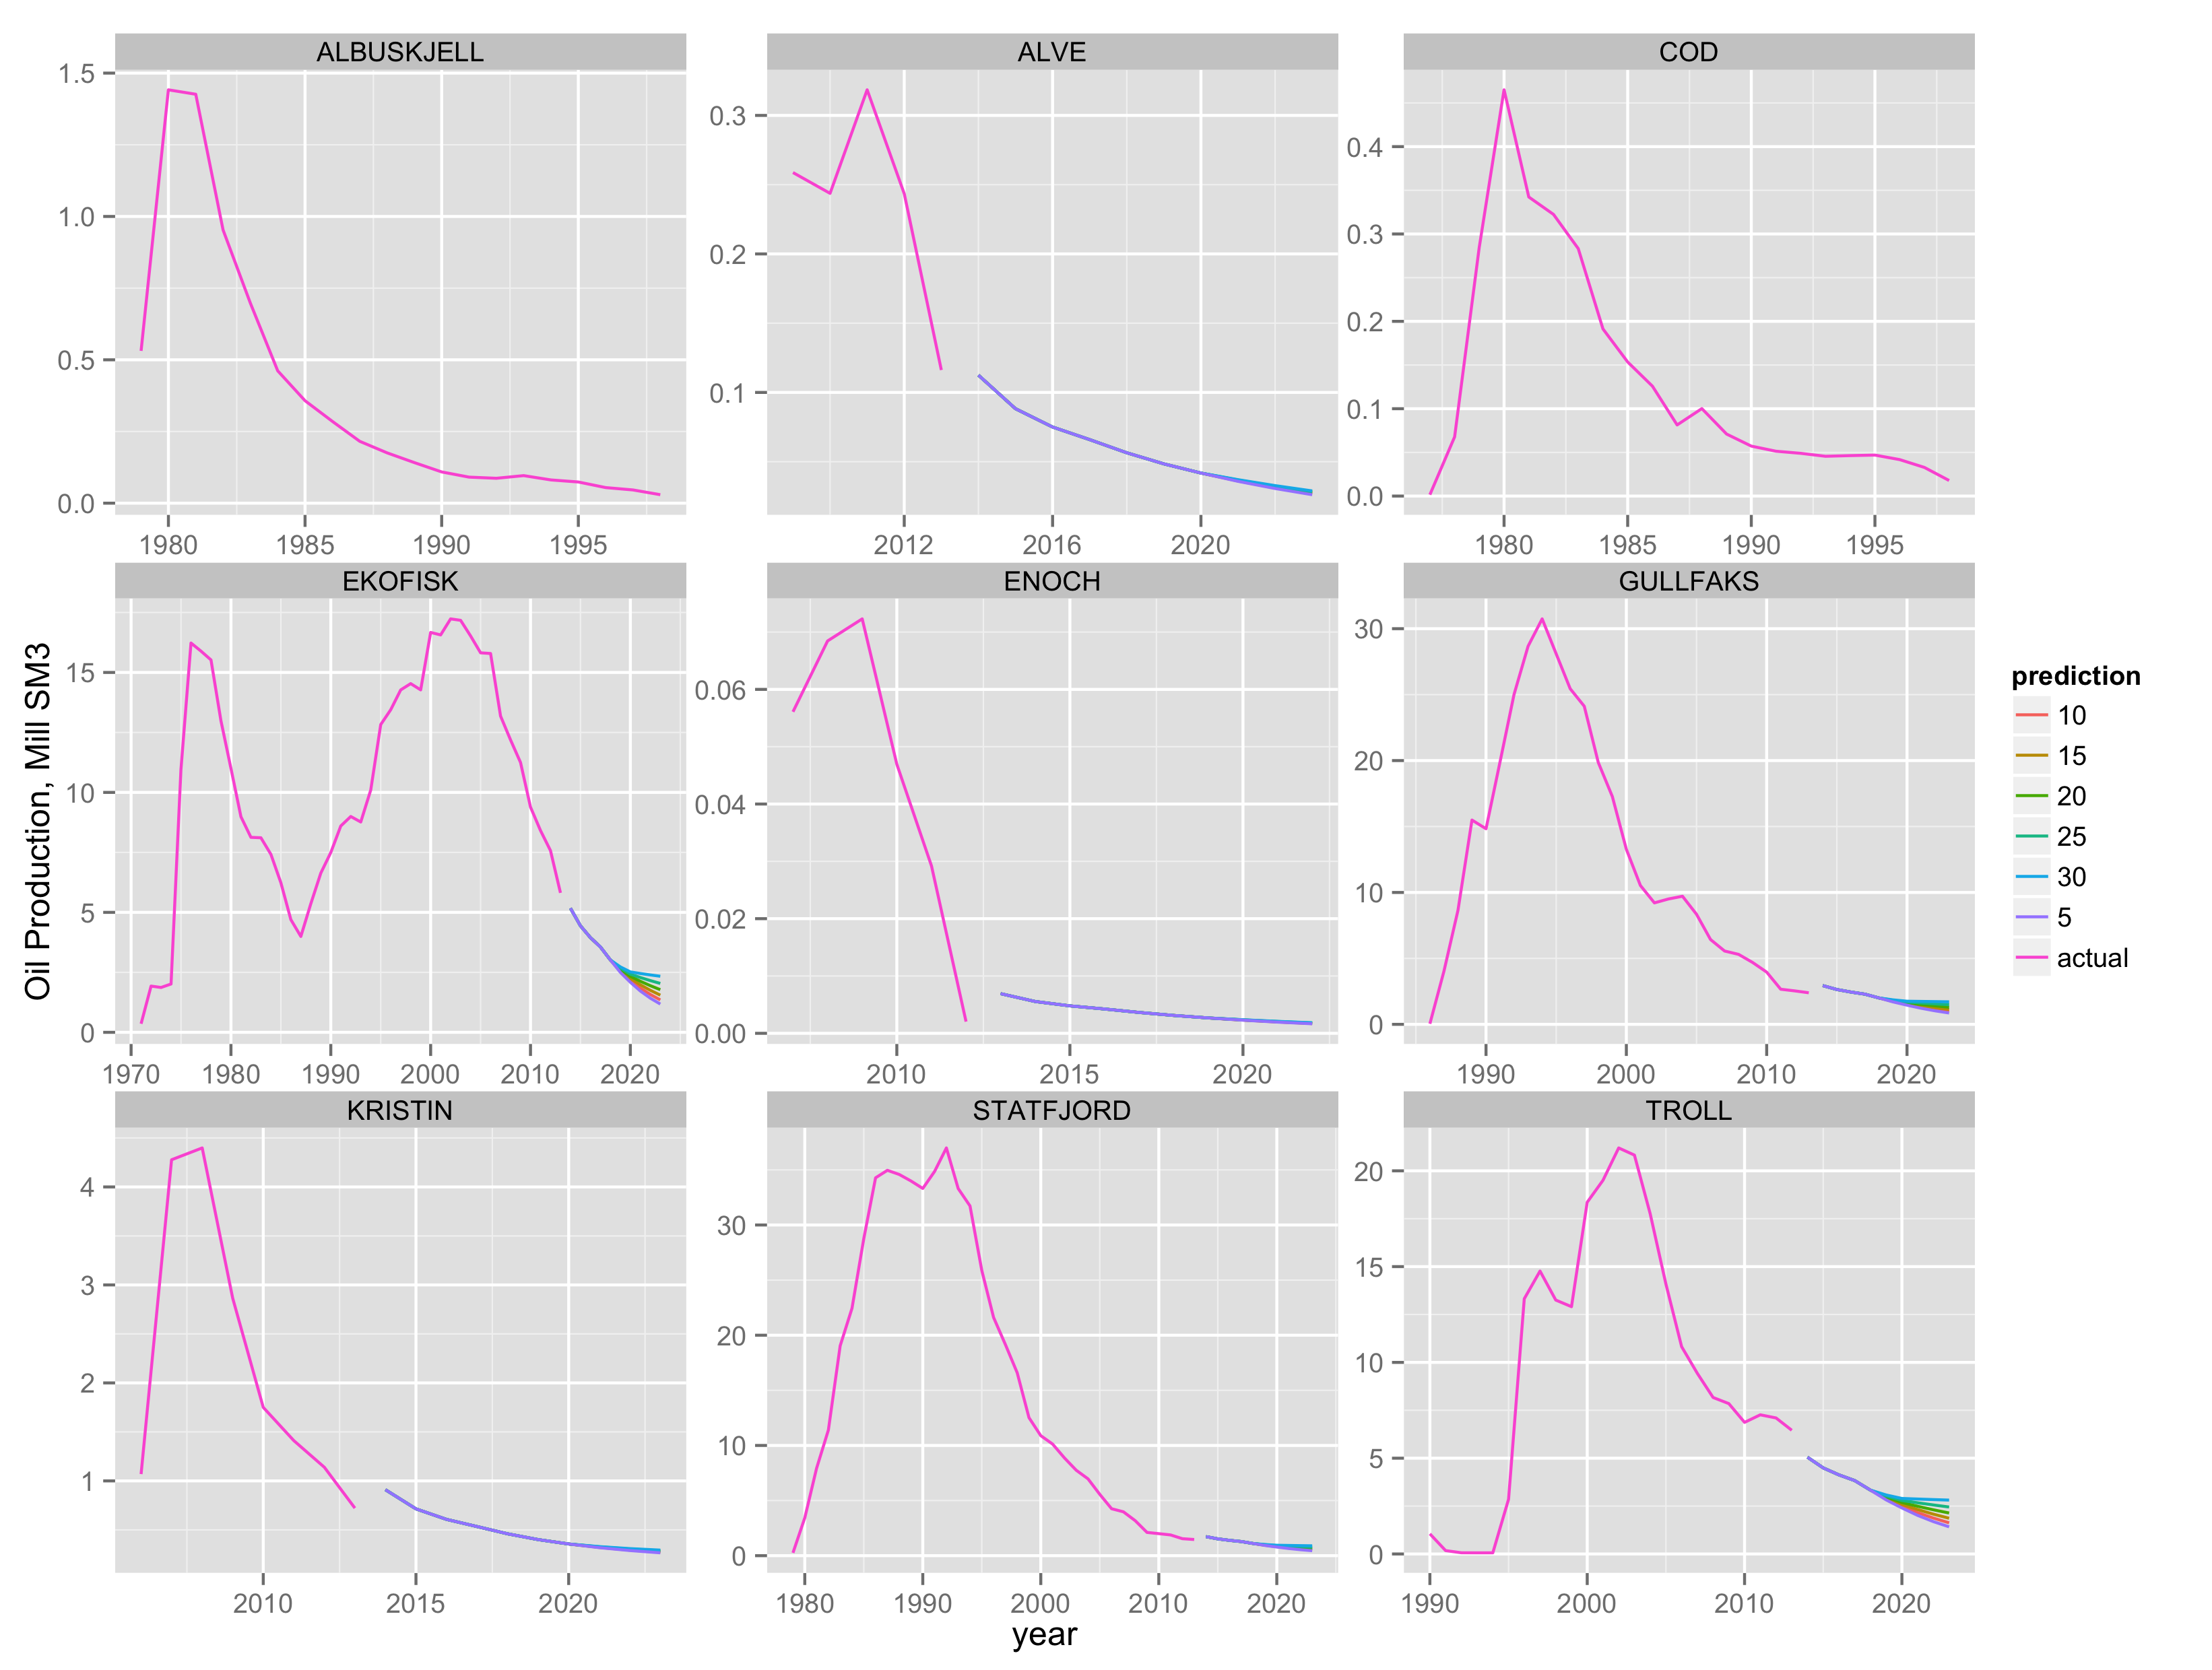
\includegraphics[width=.8\textwidth]{figures/field_lev_forecast.png}
		\caption*{}
		\label{field_lev_forecast}
	\end{figure}

\end{frame}


\begin{frame}[plain]
	\begin{figure}
		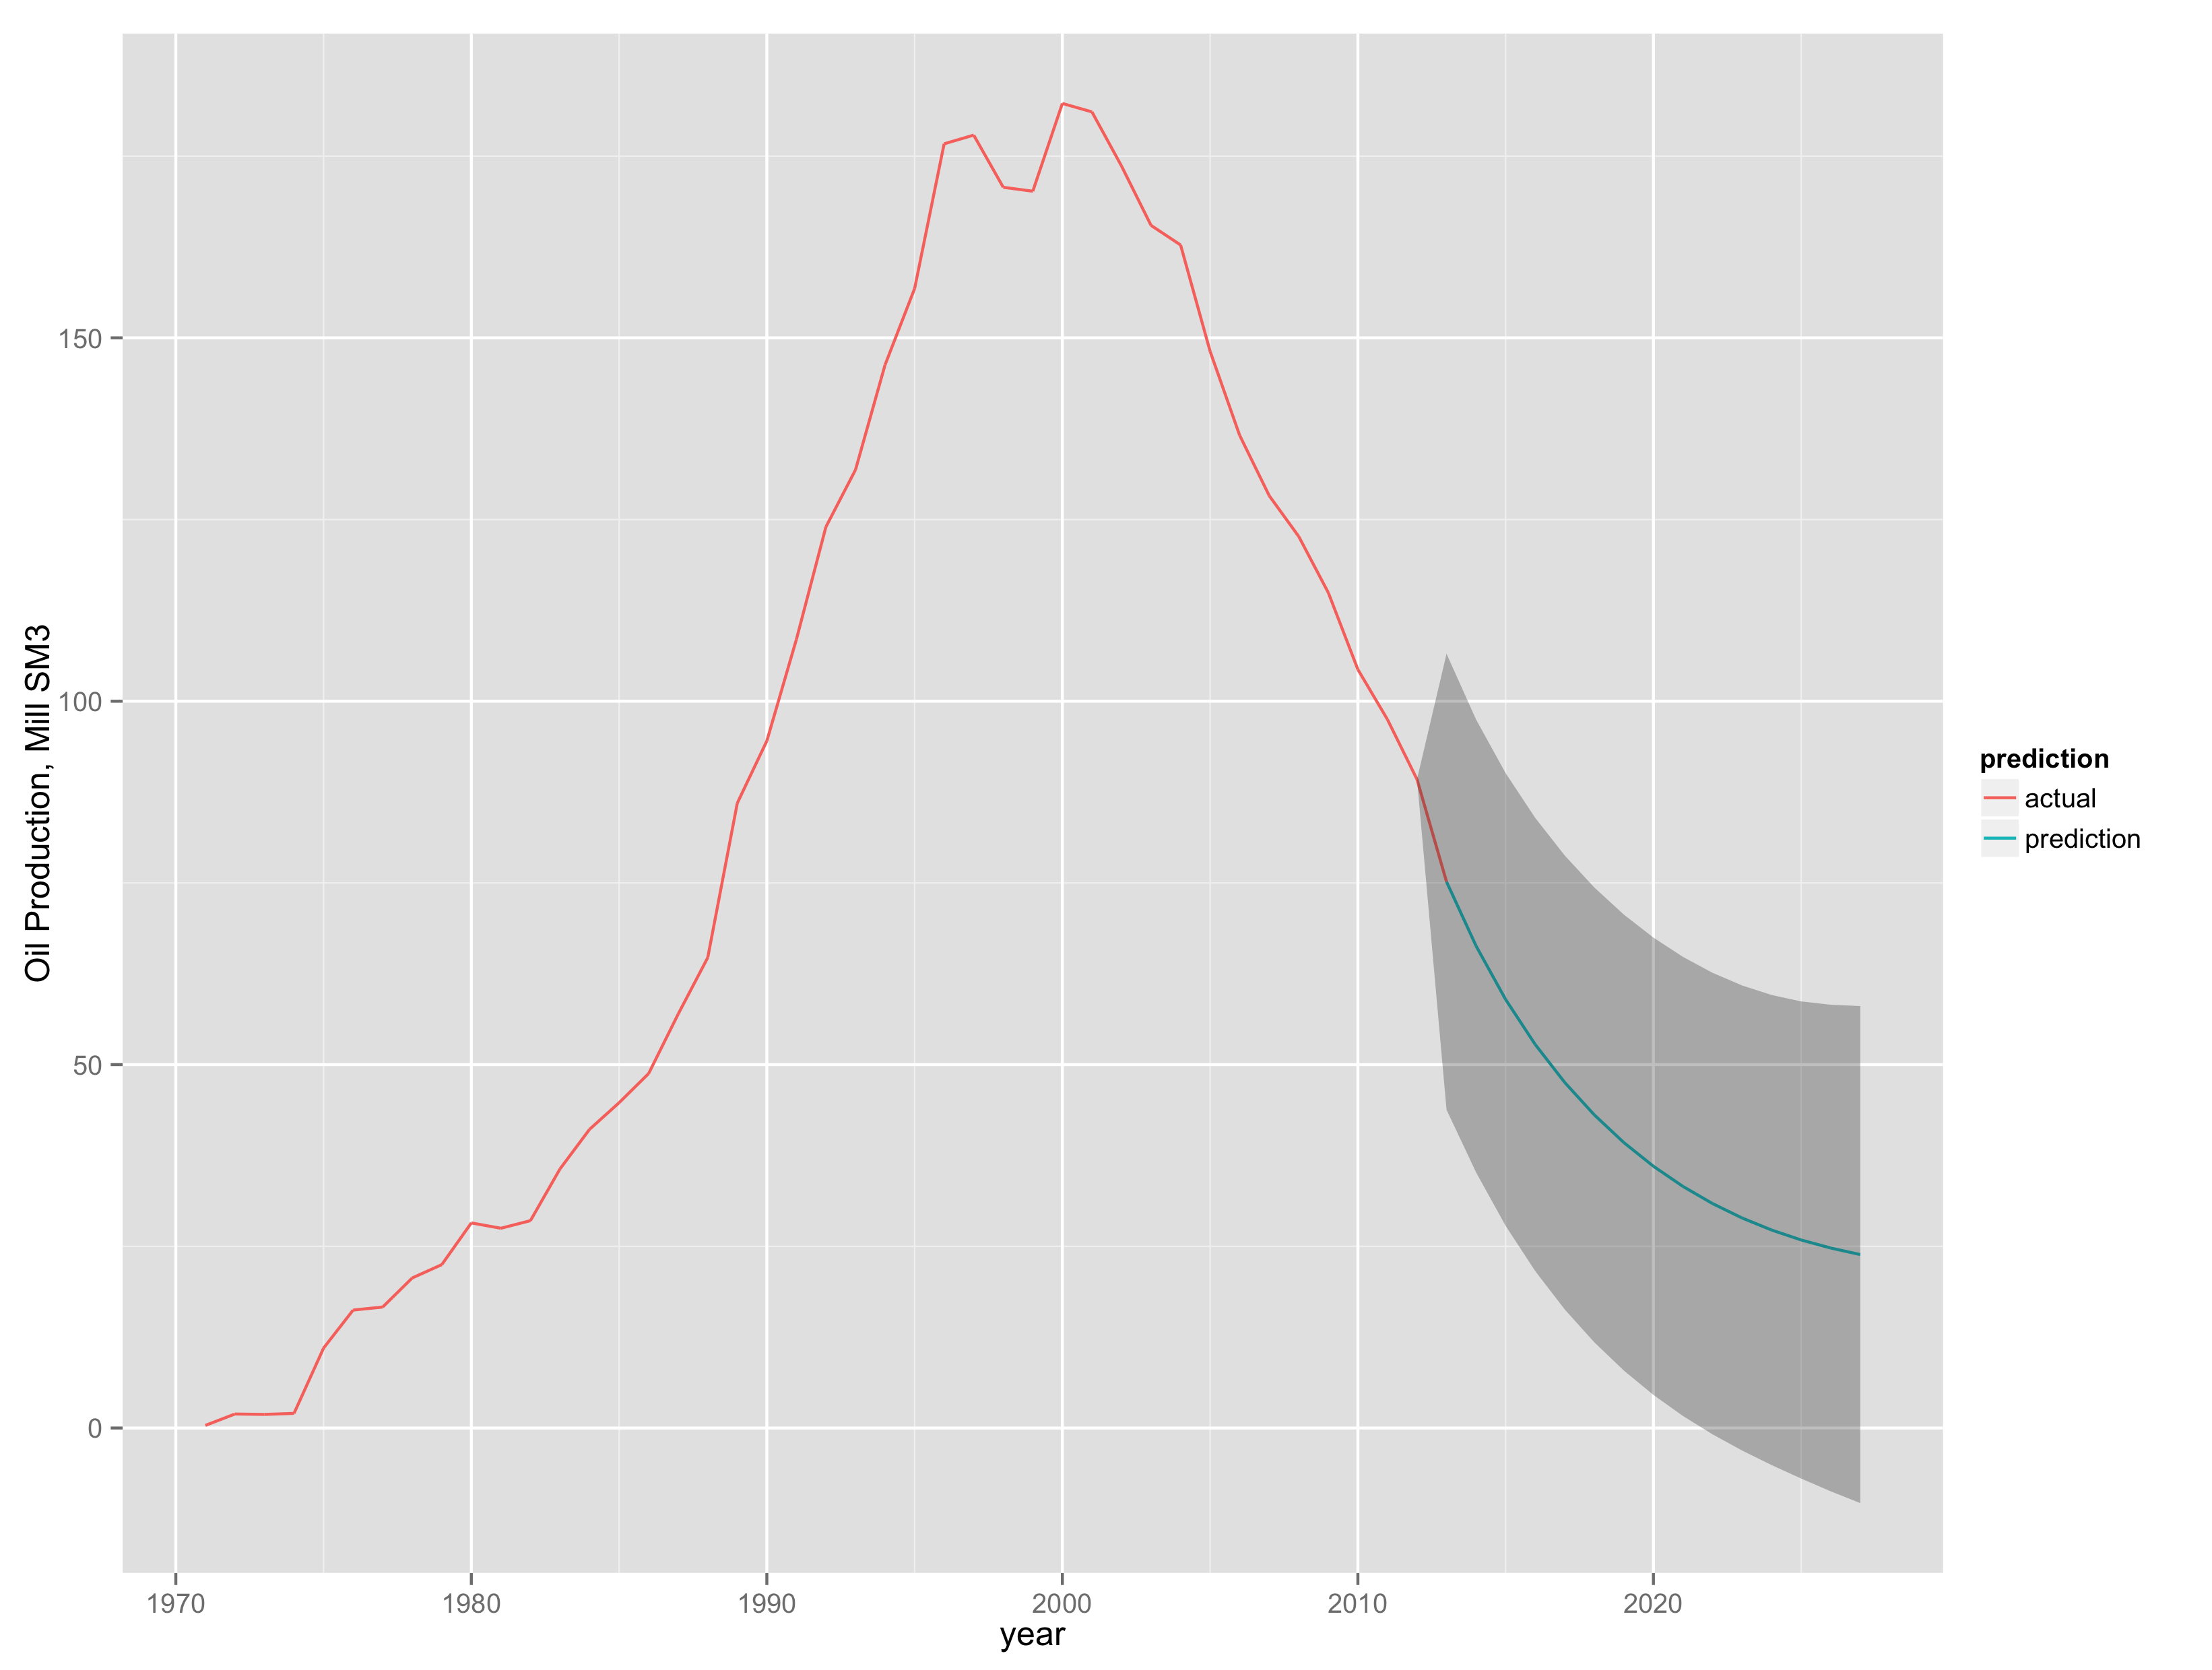
\includegraphics[width=.8\textwidth]{figures/tot_forecast.png}
		\caption*{}
		\label{tot_forecast}
	\end{figure}

\end{frame}

\begin{frame}[plain]
\begin{figure}
		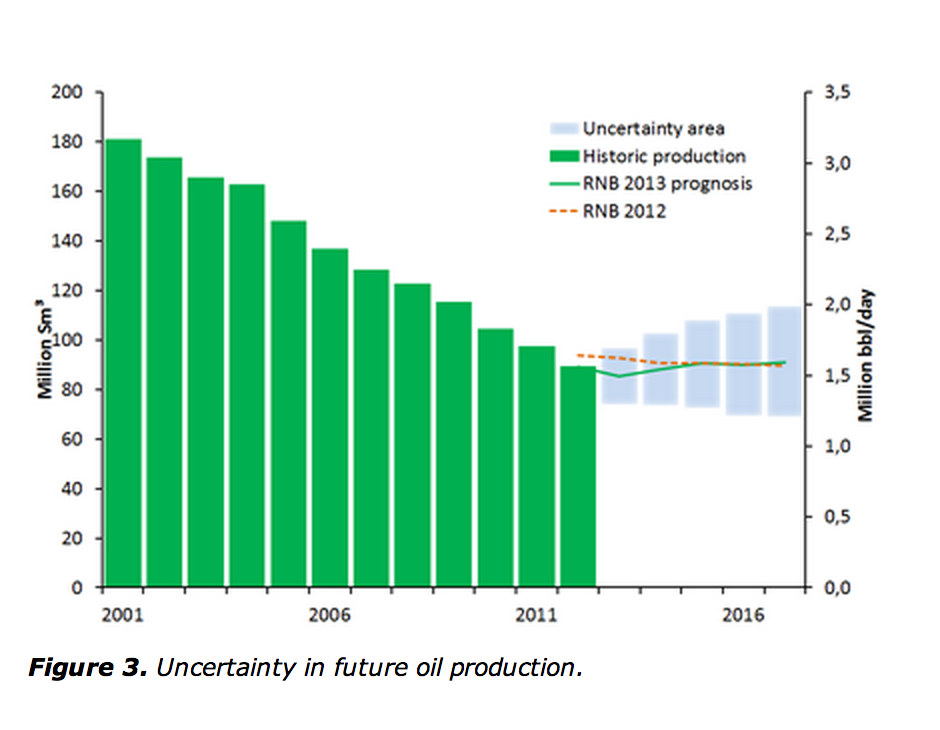
\includegraphics[width=.8\textwidth]{figures/NPD_oil_forecast.png}
		\caption*{}
		\label{NPD_oil_forecast}
	\end{figure}
\end{frame}


\begin{frame}[plain]
\begin{figure}
		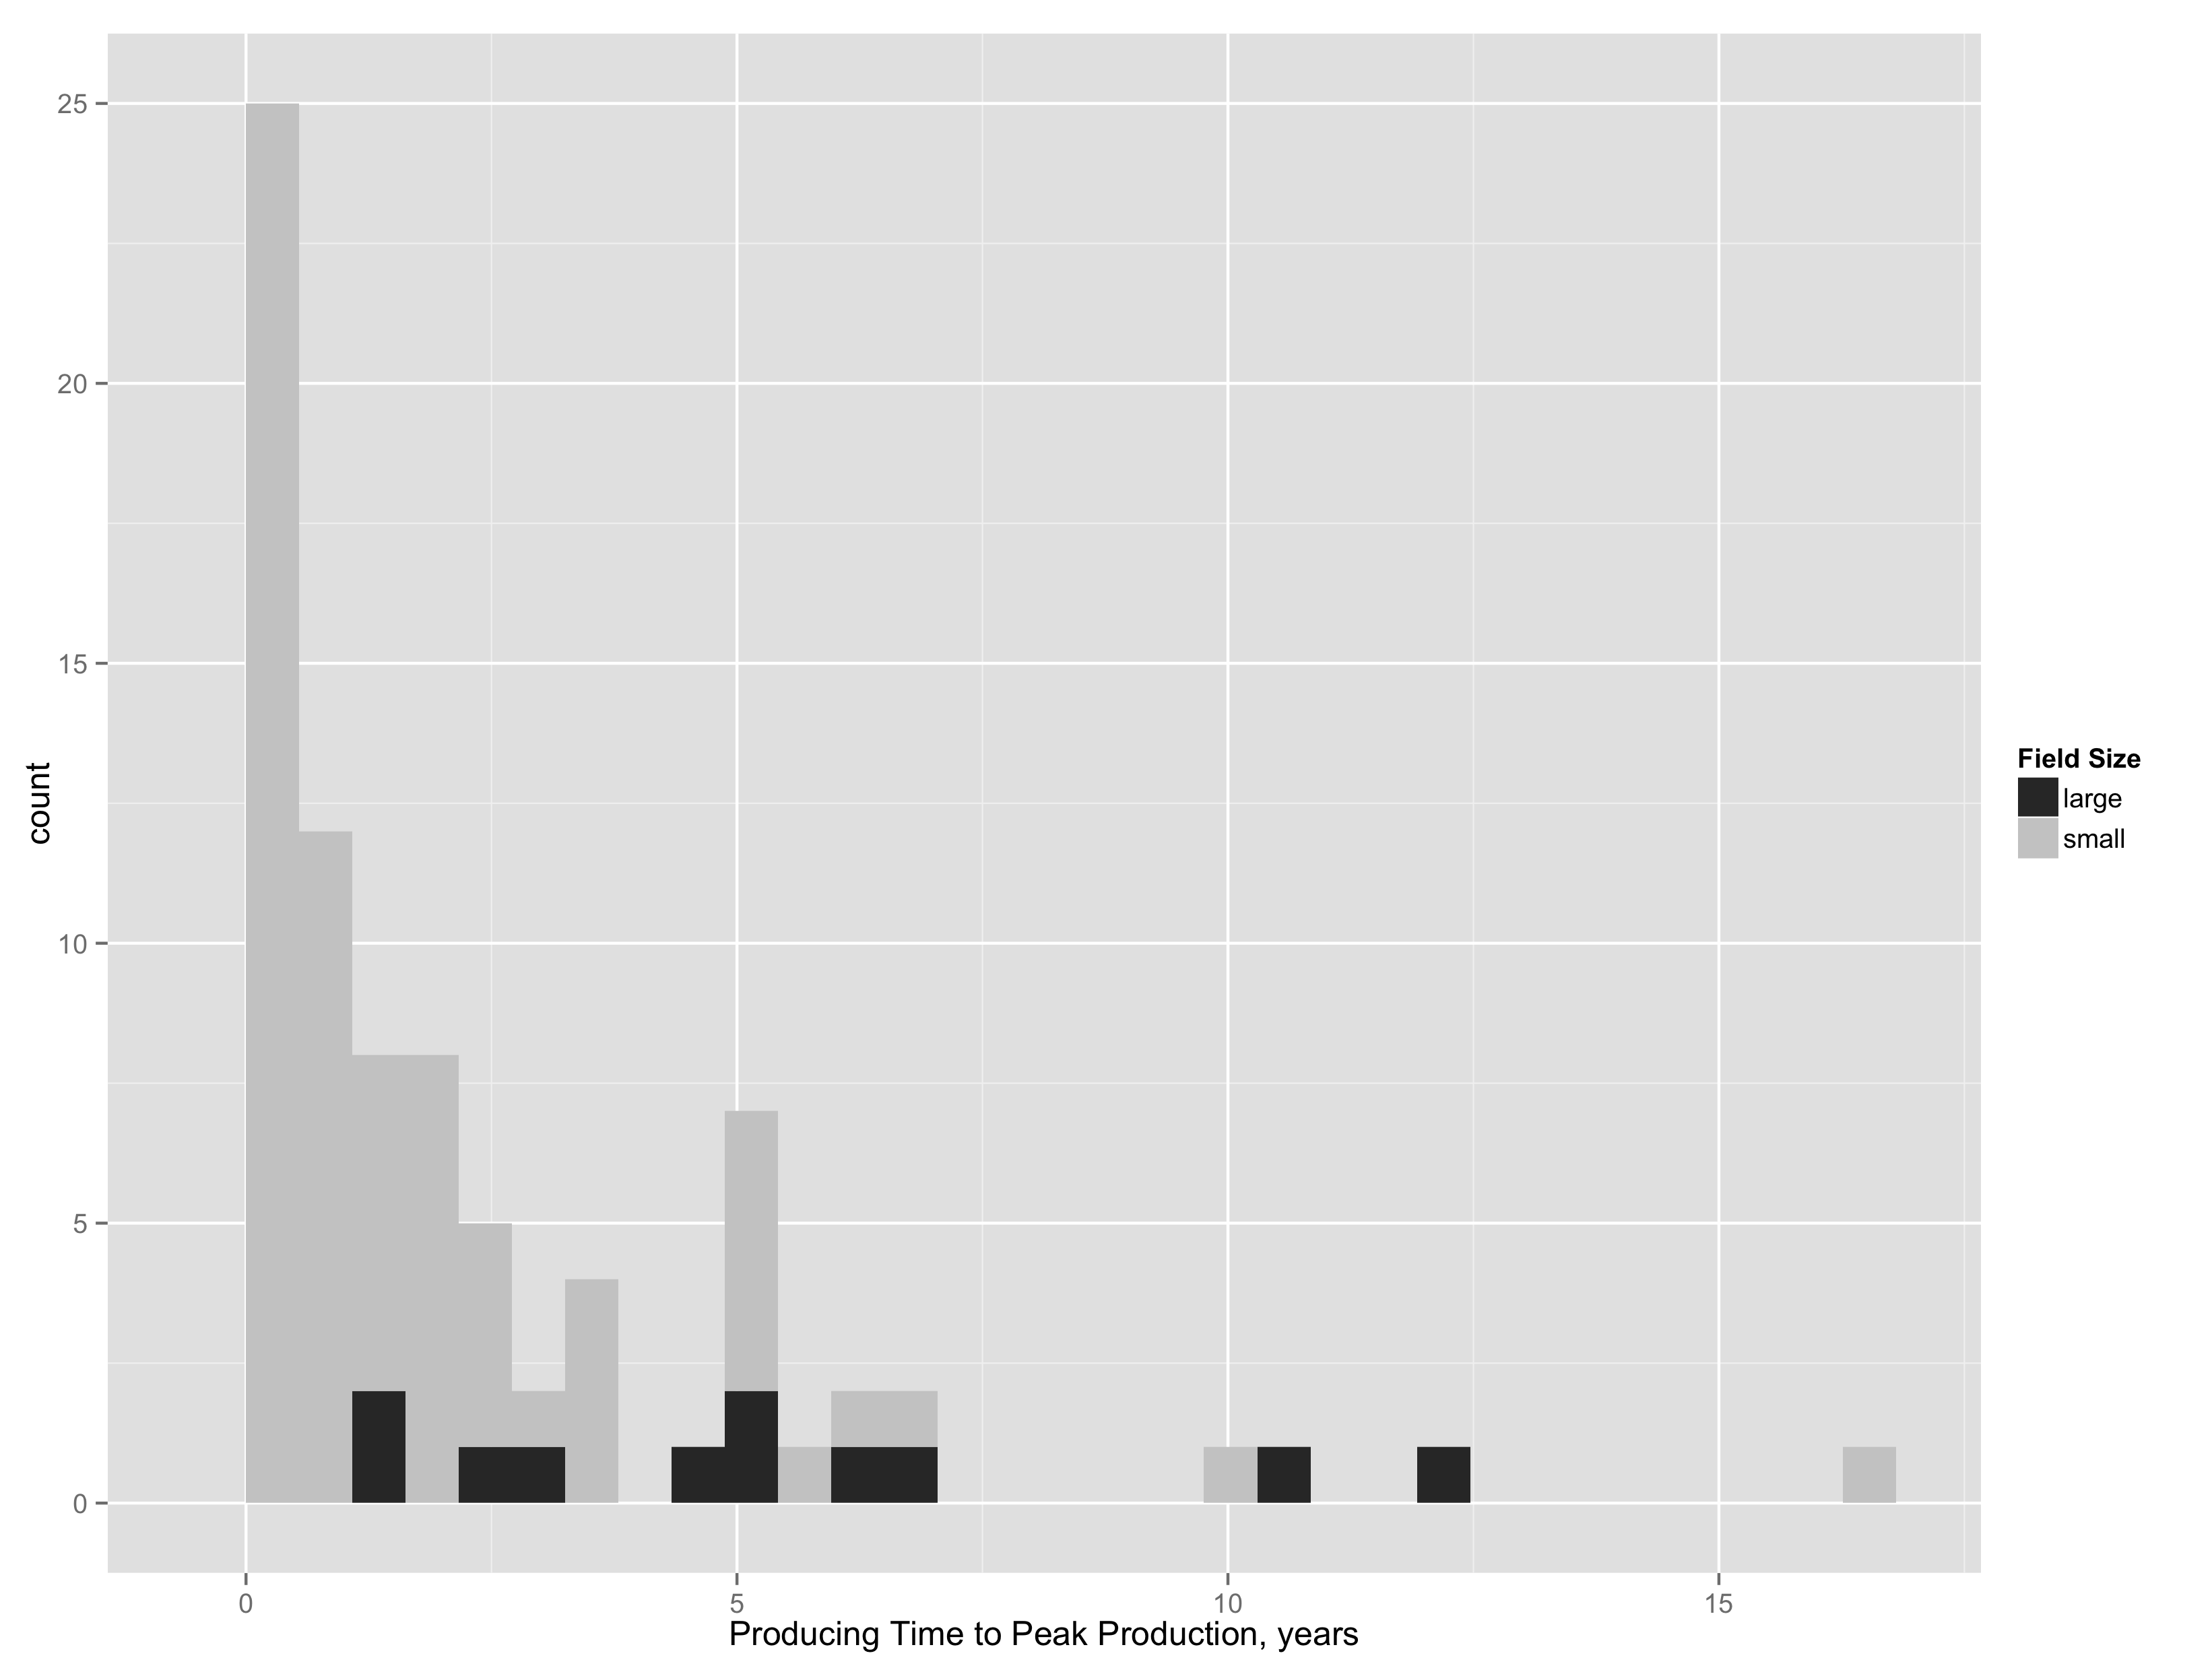
\includegraphics[width=.8\textwidth]{figures/field_time_to_peak_pres.png}
		\caption*{}
		\label{field_time_to_peak}
	\end{figure}
\end{frame}




\end{document}